% ======================================================================
%  FYS4480/FYS9480  Quantum mechanics for many-particle systems
%  Week 39, September 24-25, 2026
%  Lecture slides (Beamer).  Thursday: 2 x 45 min,  Friday: 2 x 45 min.
%
%  Sources: chapter6.tex.  Thursday: sections 6.1-6.6 (mean field,
%  variational calculus, determinants under a change of basis, the
%  Hartree-Fock equations by varying the coefficients, the density matrix and
%  the self-consistent field, Hartree-Fock in second quantization: varying
%  one orbital, <a|f|i> = 0).  Friday: section 6.7 (Thouless' theorem) and
%  section 6.10 (stability of the Hartree-Fock solution), with the Lipkin
%  model of section 6.11 as the worked illustration.
%  Exercises: suggested set for week 39 and answers to the week-38 set, at
%  the end.  Companion notebook: WeeklySlides/week39.ipynb
%  Companion program: BookPrograms/chapter06/hartreefock.py
%  Figures: ../BookFigures/chapter06/hf_fig01-03 (compile from WeeklySlides/)
%
%  Build:  pdflatex week39.tex  (twice)
%  Handout (no overlays):  replace \documentclass[...] by
%           \documentclass[handout,aspectratio=169]{beamer}
% ======================================================================
\documentclass[aspectratio=169,10pt]{beamer}

% ---------------------------------------------------------------- packages
\usepackage[utf8]{inputenc}
\usepackage[T1]{fontenc}
% \usepackage{lmodern}  % optional; uncomment if installed
\usepackage{amsmath,amssymb,bm}
\usepackage{booktabs}
\usepackage{tcolorbox}
\usepackage{listings}
\usepackage{hyperref}
\usepackage{tikz}
\usetikzlibrary{positioning,arrows.meta,decorations.markings,shapes.misc}
\usetikzlibrary{tikzmark}

% ---------------------------------------------------------------- look
\usetheme{default}
\useinnertheme{rectangles}
\setbeamertemplate{navigation symbols}{}
\definecolor{uioblue}{RGB}{18,52,86}
\definecolor{teal}{RGB}{0,128,128}
\definecolor{warm}{RGB}{181,73,36}
\definecolor{paleblue}{RGB}{232,240,248}
\definecolor{paleteal}{RGB}{228,244,244}
\definecolor{palewarm}{RGB}{252,238,230}
\setbeamercolor{structure}{fg=uioblue}
\setbeamercolor{title}{fg=uioblue}
\setbeamercolor{frametitle}{fg=uioblue,bg=white}
\setbeamercolor{section in toc}{fg=uioblue}
\setbeamercolor{alerted text}{fg=warm}
\setbeamercolor{block title}{fg=white,bg=uioblue}
\setbeamercolor{block body}{bg=paleblue}
\setbeamercolor{block title example}{fg=white,bg=teal}
\setbeamercolor{block body example}{bg=paleteal}
\setbeamerfont{frametitle}{size=\large,series=\bfseries}
\setbeamerfont{title}{size=\LARGE,series=\bfseries}
\setbeamertemplate{frametitle}{%
  \vspace*{0.6em}\insertframetitle\par
  \vspace*{-0.2em}{\color{teal}\rule{\textwidth}{0.6pt}}}
\setbeamertemplate{footline}{%
  \hbox{\begin{beamercolorbox}[wd=\paperwidth,ht=2.4ex,dp=1.2ex,leftskip=1em,rightskip=1em]{structure}%
  \footnotesize FYS4480/9480 -- Week 39 \hfill \insertsection \hfill \insertframenumber/\inserttotalframenumber
  \end{beamercolorbox}}}
\setbeamertemplate{itemize items}[circle]
\setbeamertemplate{enumerate items}[default]
\setbeamertemplate{section page}{%
  \begin{centering}
    {\usebeamerfont{section title}\usebeamercolor[fg]{title}\LARGE\bfseries\insertsection\par}
    \vspace{0.5em}{\color{teal}\rule{0.5\textwidth}{1pt}}
  \end{centering}}
\AtBeginSection[]{\frame{\sectionpage}}

% ---------------------------------------------------------------- boxes
\newcounter{thinkctr}
\newcommand{\thinkq}[2]{%
  \stepcounter{thinkctr}%
  \begin{tcolorbox}[colback=palewarm,colframe=warm,title={\bfseries Pause to think \#\thethinkctr\hfill\mdseries\small(about #1 min -- discuss with your neighbour)},fonttitle=\bfseries]
  #2
  \end{tcolorbox}}
\newcommand{\thinka}[1]{%
  \begin{tcolorbox}[colback=paleteal,colframe=teal,title={\bfseries Answer to pause \#\thethinkctr}]
  #1
  \end{tcolorbox}}
\newcommand{\mbbox}[1]{%
  \begin{tcolorbox}[colback=paleblue,colframe=uioblue,title={\bfseries Many-body connection}]
  #1
  \end{tcolorbox}}
\newcommand{\qcbox}[1]{%
  \begin{tcolorbox}[colback=paleteal,colframe=teal,title={\bfseries Quantum computing connection}]
  #1
  \end{tcolorbox}}

% ---------------------------------------------------------------- code
\lstset{language=Python,basicstyle=\ttfamily\scriptsize,
  keywordstyle=\color{uioblue}\bfseries,commentstyle=\color{teal},
  stringstyle=\color{warm},showstringspaces=false,columns=fullflexible,
  frame=single,rulecolor=\color{paleblue},backgroundcolor=\color{white},
  breaklines=true}

% ---------------------------------------------------------------- macros
\newcommand{\ket}[1]{\vert #1\rangle}
\newcommand{\bra}[1]{\langle #1\vert}
\newcommand{\braket}[2]{\langle #1\vert #2\rangle}
\newcommand{\ketbra}[2]{\vert #1\rangle\langle #2\vert}
\newcommand{\element}[3]{\langle #1\vert #2\vert #3\rangle}
\newcommand{\dd}{\mathrm{d}}
\newcommand{\Det}[1]{\vert\bm{#1}\vert}
\DeclareMathOperator{\tr}{tr}
\DeclareMathOperator{\sgn}{sgn}
\newcommand{\bigO}{\mathcal{O}}
% normal ordering with respect to the reference determinant |c>
\newcommand{\nc}[1]{\bigl\{#1\bigr\}}
% Wick contraction lines, as in the book (book.tex).
\newcommand{\wmark}[2]{\tikzmarknode{#1}{\vphantom{a_p^{\dagger}}#2}}
\newcommand{\wline}[3][2.4ex]{%
  \begin{tikzpicture}[overlay,remember picture]
    \draw[thin] ([yshift=0.7ex]#2.north) -- ++(0,#1)
                -| ([yshift=0.7ex]#3.north);
  \end{tikzpicture}}
\newcommand{\wlineb}[3][2.4ex]{%
  \begin{tikzpicture}[overlay,remember picture]
    \draw[thin] ([yshift=-0.5ex]#2.south) -- ++(0,-#1)
                -| ([yshift=-0.5ex]#3.south);
  \end{tikzpicture}}
\newcommand{\wstrut}[1][4.6ex]{\vphantom{\rule{0pt}{#1}}}

% ---------------------------------------------------------------- diagrams
% Goldstone-style diagrams for the projected FCI equations. Time runs
% upward. All lines are drawn from bottom to top; a particle line carries an
% upward arrow, a hole line a downward arrow, at the midpoint.
\tikzset{
  pline/.style={thick,postaction={decorate},decoration={markings,mark=at position 0.55 with {\arrow{Stealth[length=5pt]}}}},
  hline/.style={thick,postaction={decorate},decoration={markings,mark=at position 0.55 with {\arrowreversed{Stealth[length=5pt]}}}},
  vint/.style={dashed,thick},
  vtx/.style={circle,fill=uioblue,inner sep=1.4pt},
  fvtx/.style={cross out,draw=uioblue,thick,minimum size=5pt,inner sep=0pt},
  amp/.style={line width=2.4pt,uioblue},
  dlab/.style={font=\scriptsize},
  every picture/.style={scale=0.8,baseline=(current bounding box.center)}
}

\graphicspath{{../BookFigures/}{./}}

% ---------------------------------------------------------------- title
\title{Hartree-Fock theory: from the variational principle to $\langle a\vert\hat{f}\vert i\rangle=0$, Thouless' theorem, and the stability of the mean field}
\subtitle{FYS4480/FYS9480 -- Week 39, September 24--25, 2026}
\author{Morten Hjorth-Jensen}
\institute{Department of Physics and Center for Computing in Science Education,\\
University of Oslo, Norway}
\date{}

\begin{document}

\begin{frame}[plain]
  \vspace*{0.2em}{\setbeamerfont{title}{size=\Large,series=\bfseries}\titlepage}
  \vfill
  \begin{center}\scriptsize
  Thursday September 24: why a mean field; variational calculus and Lagrange multipliers; determinants under a change of basis; the Hartree-Fock equations by varying the coefficients; the density matrix and the self-consistent field; Brillouin's theorem; Hartree-Fock in second quantization -- varying one orbital, $\ket{\Phi_0}+\eta\,a_a^{\dagger}a_i\ket{\Phi_0}$, and the equation $\langle a\vert\hat{f}\vert i\rangle=0$\\
  Friday September 25: Thouless' theorem -- what a nearby determinant is, and its proof; the stability of the Hartree-Fock solution -- the energy to second order, the stability matrix, stationary versus minimal, and the Lipkin model as an explicit instability\\[0.2em]
  Reading: these slides; lecture notes chapter 6, sections 6.1--6.7 and 6.10--6.11; Szabo and Ostlund chapter 3; Shavitt and Bartlett chapter 4. Code: \texttt{WeeklySlides/week39.ipynb}, \texttt{BookPrograms/chapter06/hartreefock.py}
  \end{center}
\end{frame}

\begin{frame}[shrink=5]{Plan for week 39}
  \scriptsize
  \begin{block}{Thursday September 24, $2\times45$ min}
    \begin{itemize}
      \item Why a mean field; the two ingredients of Hartree-Fock theory; $E^{\mathrm{HF}}\ge E_0$ (section 6.1)
      \item Variational calculus with Lagrange multipliers; determinants under a linear change of basis and the invariance under unitary mixing of the occupied orbitals (sections 6.2--6.3)
      \item The Hartree-Fock equations by varying the expansion coefficients; the Fock matrix; a nonlinear eigenvalue problem (section 6.4)
      \item The density matrix and the self-consistent field; convergence of the energy versus convergence of the orbitals; Brillouin's theorem (section 6.5)
      \item Hartree-Fock in second quantization: varying one orbital is adding a $1p$-$1h$ determinant; the energy to first order with complex $\eta$; the normal-ordered Hamiltonian gives $\langle a\vert\hat{f}\vert i\rangle=0$, and how that becomes the eigenvalue problem (section 6.6)
    \end{itemize}
  \end{block}
  \begin{block}{Friday September 25, $2\times45$ min}
    \begin{itemize}
      \item Thouless' theorem: every determinant not orthogonal to $\ket{c}$ is $e^{\hat{T}}\ket{c}$ with $\hat{T}$ a sum of $1p$-$1h$ operators; the three steps of the proof; what it buys us (section 6.7)
      \item Stability: stationary is not minimal; the energy to second order; the stability matrix $\hat{M}$ with blocks $\Delta$, $A$, $B$; the criterion; $\hat{M}$ is the RPA matrix (section 6.10); the Lipkin model as an explicit instability, the pairing model as stable but useless (section 6.11)
      \item Exercises: suggested set for week 39, and answers to the week-38 set (last frames)
    \end{itemize}
  \end{block}
\end{frame}

% ======================================================================
\section{Thursday, lecture 1: Mean field, variations and the Hartree-Fock equations}
% ======================================================================

\begin{frame}[shrink=1]{Where we are, and the map of the week}
  \footnotesize
  \begin{columns}[T]
    \column{0.52\textwidth}
    \begin{block}{Chapter 5 said}
      The exact ground state is $\sum_K C_K\ket{\Phi_K}$ over exponentially many determinants, and we cannot afford it. In a Hartree-Fock basis the reference decouples from the singles, and every truncation improves. \alert{So: which single determinant is best?}
    \end{block}
    \begin{block}{Chapter 6 answers, three times}
      \begin{enumerate}
        \item Vary the \emph{expansion coefficients} of the orbitals with Lagrange multipliers $\to$ the eigenvalue problem $\bm{h}^{\mathrm{HF}}\bm{C}=\bm{\epsilon}\bm{C}$ (6.4, Thursday)
        \item Vary \emph{one orbital} towards one unoccupied orbital $\to$ $\langle a\vert\hat{f}\vert i\rangle=0$ (6.6, Thursday)
        \item Vary the \emph{determinant} itself, with Thouless' theorem telling us what a nearby determinant is $\to$ the same, and the second-order term that decides stability (6.7, 6.10, Friday)
      \end{enumerate}
    \end{block}
    \column{0.46\textwidth}
    \mbbox{Hartree-Fock is the foundation of everything after it: perturbation theory expands about it, coupled cluster exponentiates corrections to it, truncated CI is measured against it, and TDA/RPA turn out to be its second derivative. The condition $f_{ai}=0$ derived today is why the singles are absent from the leading orders of all of them.}
    \vspace{0.1em}
    \footnotesize Notation as in weeks 35--38: $i,j,\dots\le F$ holes, $a,b,\dots>F$ particles, $p,q,\dots$ any; $\element{pq}{\hat{v}}{rs}$ antisymmetrised.
  \end{columns}
\end{frame}

\begin{frame}{Why a mean field? (section 6.1)}
  \footnotesize
  Instead of adding determinants we keep exactly one and ask which one is best.
  \begin{block}{Hartree-Fock theory in two ingredients}
    A single-particle basis defined by its own eigenvalue problem,
    \[
      \hat{h}^{\mathrm{HF}}\psi_\alpha=\varepsilon_\alpha\psi_\alpha,\qquad
      \hat{h}^{\mathrm{HF}}=\hat{t}+\hat{u}_{\mathrm{ext}}+\hat{u}^{\mathrm{HF}},
    \]
    and the prescription for the still unknown one-body potential $\hat{u}^{\mathrm{HF}}$: choose it such that $E^{\mathrm{HF}}=\bra{\Phi_0}\hat{H}\ket{\Phi_0}$ is stationary, with $\ket{\Phi_0}$ the determinant of the $N$ lowest solutions.
  \end{block}
  \begin{itemize}
    \item The variational principle guarantees $E^{\mathrm{HF}}\ge E_0$: an upper bound, like every Ritz value of week 38 -- here with the \emph{orbitals} as parameters and the expansion frozen at one term.
    \item We shall find that $\hat{h}^{\mathrm{HF}}$ is exactly the operator $\hat{f}$ of the normal-ordered Hamiltonian of week 37,
    \[
      \element{p}{\hat{h}^{\mathrm{HF}}}{q}=\element{p}{\hat{f}}{q}=\element{p}{\hat{t}+\hat{u}_{\mathrm{ext}}}{q}+\sum_{i\le F}\element{pi}{\hat{v}}{qi},
      \qquad
      \element{p}{\hat{u}^{\mathrm{HF}}}{q}=\sum_{i\le F}\element{pi}{\hat{v}}{qi}.
    \]
    \item This is the whole content of the mean-field idea: \alert{the interaction summed over the other fermions is an effective one-body field} in which a given fermion moves. It depends on which states are occupied (\emph{medium dependence}) and on the interaction: different interactions give different mean fields at the same density.
    \item For atoms and molecules $\hat{u}_{\mathrm{ext}}$ is the attraction of the nuclei. A nucleus has none: it is self-bound, and the entire one-body field must be generated by the sum over the occupied states.
  \end{itemize}
\end{frame}

\begin{frame}{Variational calculus and Lagrange multipliers (section 6.2)}
  \small
  The machinery of week 38, in its simplest setting: one particle, $E=\int\psi^{*}\hat{H}\psi\,\dd^3r$ with $\int\psi^{*}\psi\,\dd^3r=1$ and $\hat{H}=-\frac12\nabla^2+V$. Integrating the kinetic term by parts, the constrained variation is
  \[
    \delta\Bigl\{\int\Bigl(\tfrac12\nabla\psi^{*}\cdot\nabla\psi+V\psi^{*}\psi-\lambda\psi^{*}\psi\Bigr)\dd^3r\Bigr\}=0 .
  \]
  With $f=\frac12(\psi_x^{*}\psi_x+\psi_y^{*}\psi_y+\psi_z^{*}\psi_z)+V\psi^{*}\psi-\lambda\psi^{*}\psi$, the Euler-Lagrange equation for $\psi^{*}$,
  \[
    \frac{\partial f}{\partial\psi^{*}}-\frac{\partial}{\partial x}\frac{\partial f}{\partial\psi_x^{*}}-\frac{\partial}{\partial y}\frac{\partial f}{\partial\psi_y^{*}}-\frac{\partial}{\partial z}\frac{\partial f}{\partial\psi_z^{*}}=0
    \qquad\Longrightarrow\qquad
    -\tfrac12\nabla^2\psi+V\psi=\lambda\psi .
  \]
  \begin{itemize}
    \item The multiplier is the energy and the stationarity condition is the Schr\"odinger equation. \alert{The pattern}: a constrained variation produces an eigenvalue problem, and the multiplier enforcing normalisation is the eigenvalue. In FCI the unknowns were the coefficients $C_K$ and the constraint $\sum|C_K|^2=1$; here the unknown is a function and the constraint an integral.
    \item In Hartree-Fock the unknowns are $N$ orbitals and the constraints are the orthonormality integrals $\braket{i}{j}=\delta_{ij}$. Naively that is $N(N+1)/2$ multipliers; the next slide explains why one per orbital is enough.
  \end{itemize}
\end{frame}

\begin{frame}{Pause to think: multipliers}
  \thinkq{3}{
  \begin{enumerate}
    \item In the one-particle example, why does the multiplier turn out to be the energy, and not some other number?
    \item For $N$ orbitals there are $N(N+1)/2$ independent orthonormality constraints $\braket{i}{j}=\delta_{ij}$, but the Hartree-Fock equations of section 6.4 carry only $N$ multipliers $\epsilon_i$. What has been thrown away, and why is that allowed?
  \end{enumerate}}
\end{frame}

\begin{frame}{Answer}
  \thinka{
  \begin{enumerate}
    \item Multiply the Euler-Lagrange equation $-\frac12\nabla^2\psi+V\psi=\lambda\psi$ by $\psi^{*}$ and integrate: $\lambda\int\psi^{*}\psi=\int\psi^{*}\hat{H}\psi=E$. With the constraint $\int\psi^{*}\psi=1$ the multiplier is the expectation value of $\hat{H}$ in the stationary state -- and since the stationary states are the eigenstates, that expectation value is the eigenvalue. The same argument gives $\lambda=E$ for the FCI coefficients in week 38.
    \item The off-diagonal constraints $\braket{i}{j}=0$, $i\ne j$, have been thrown away. The full set of multipliers is a Hermitian matrix $\epsilon_{ij}$ and the equations read $\hat{h}^{\mathrm{HF}}\psi_i=\sum_j\epsilon_{ij}\psi_j$. But the energy, and the determinant up to a phase, are invariant under a unitary mixing of the occupied orbitals (next slide), so we may rotate the occupied orbitals until $\epsilon_{ij}$ is diagonal. That rotation costs nothing and leaves one multiplier per orbital: the \emph{canonical} Hartree-Fock orbitals. The diagonal form is a convention, not a consequence of the variation -- a point that returns in section 6.6.
  \end{enumerate}}
\end{frame}

\begin{frame}{Determinants under a linear change of basis (section 6.3)}
  \footnotesize
  A determinant is linear in each column (and in each row) separately,
  \[
    \begin{vmatrix}\alpha_1b_{11}+\alpha_2b_{12} & a_{12}\\ \alpha_1b_{21}+\alpha_2b_{22} & a_{22}\end{vmatrix}
    =\alpha_1\begin{vmatrix}b_{11} & a_{12}\\ b_{21} & a_{22}\end{vmatrix}+\alpha_2\begin{vmatrix}b_{12} & a_{12}\\ b_{22} & a_{22}\end{vmatrix},
    \qquad\text{and in general }\det(\bm{B}\bm{C})=\det\bm{B}\,\det\bm{C}.
  \]
  Expand new orbitals in a fixed orthonormal basis, $\psi_p(x)=\sum_\lambda C_{p\lambda}\phi_\lambda(x)$. The Slater determinant of the $\psi$'s is
  \[
    \frac{1}{\sqrt{N!}}
    \begin{vmatrix}
      \sum_\lambda C_{p\lambda}\phi_\lambda(x_1) & \cdots & \sum_\lambda C_{p\lambda}\phi_\lambda(x_N)\\
      \vdots & & \vdots\\
      \sum_\lambda C_{t\lambda}\phi_\lambda(x_1) & \cdots & \sum_\lambda C_{t\lambda}\phi_\lambda(x_N)
    \end{vmatrix}
    =\det(\bm{C})\,\Phi(\phi),
  \]
  with $\Phi(\phi)$ the determinant of the original basis functions (rows $=$ orbitals, columns $=$ particles, as in chapter 2). Two consequences, used constantly:
  \begin{itemize}
    \item \textbf{Orthonormality is preserved by a unitary $\bm{C}$}: $\bm{w}_j^{\dagger}\bm{w}_i=\bm{v}_j^{\dagger}\bm{U}^{\dagger}\bm{U}\bm{v}_i=\delta_{ij}$. A unitary change of coefficients never spoils the basis.
    \item \textbf{A determinant is invariant, up to a phase, under any unitary mixing of its occupied orbitals}: it knows only which $N$-dimensional subspace they span. The Hartree-Fock solution is a statement about a \alert{subspace}; the individual orbitals are fixed only by the convention that the Fock matrix be diagonal. Today's second derivation will use the same fact from the other side: a variation \emph{inside} the occupied subspace does nothing.
  \end{itemize}
\end{frame}

\begin{frame}{The energy functional in terms of the coefficients (section 6.4)}
  \footnotesize
  The energy of a single determinant is the functional of week 34, $E_{\mathrm{ref}}$ of week 37:
  \[
    E[\Phi]=\sum_{\mu=1}^{N}\element{\mu}{\hat{h}_0}{\mu}+\frac12\sum_{\mu\nu=1}^{N}\element{\mu\nu}{\hat{v}}{\mu\nu}_{\mathrm{AS}} .
  \]
  Insert $\psi_i=\sum_\alpha C_{i\alpha}\phi_\alpha$ (Greek indices over the whole fixed basis, Latin over the $N$ occupied orbitals):
  \begin{block}{$E$ as a function of the coefficients}
    \[
      E[\Phi^{\mathrm{HF}}]=\sum_{i=1}^{N}\sum_{\alpha\beta}C_{i\alpha}^{*}C_{i\beta}\element{\alpha}{\hat{h}_0}{\beta}
      +\frac12\sum_{i,j=1}^{N}\sum_{\alpha\beta\gamma\delta}C_{i\alpha}^{*}C_{j\beta}^{*}C_{i\gamma}C_{j\delta}\element{\alpha\beta}{\hat{v}}{\gamma\delta}_{\mathrm{AS}} .
    \]
  \end{block}
  \begin{itemize}
    \item The coefficients are not free: $\braket{i}{j}=\delta_{ij}=\sum_\alpha C_{i\alpha}^{*}C_{j\alpha}$. Introduce one multiplier $\epsilon_i$ per occupied orbital (pause \#1) and make
    \[
      F[\Phi^{\mathrm{HF}}]=E[\Phi^{\mathrm{HF}}]-\sum_{i=1}^{N}\epsilon_i\sum_\alpha C_{i\alpha}^{*}C_{i\alpha}
    \]
    stationary. $C$ and $C^{*}$ may be varied independently (real and imaginary parts are two independent real variations): $\partial F/\partial C_{i\alpha}^{*}=0$.
    \item Compare with FCI: there $E$ was \emph{quadratic} in the unknowns and the condition linear. Here $E$ is \emph{quartic}, and the condition will be an eigenvalue problem whose matrix depends on its own solution.
  \end{itemize}
\end{frame}

\begin{frame}{Carrying out the variation}
  \footnotesize
  Differentiate with respect to $C_{i\alpha}^{*}$. The one-body term gives $\sum_\beta C_{i\beta}\element{\alpha}{\hat{h}_0}{\beta}$. In the two-body term $C_{i\alpha}^{*}$ appears twice -- as $C_{i\alpha}^{*}$ and as $C_{j\beta}^{*}$ with $j=i$ -- with equal contributions by the symmetry of $\element{\alpha\beta}{\hat{v}}{\gamma\delta}_{\mathrm{AS}}$ under the simultaneous interchange of both pairs; they cancel the $\frac12$:
  \[
    \sum_\beta C_{i\beta}\element{\alpha}{\hat{h}_0}{\beta}
    +\sum_{j=1}^{N}\sum_{\beta\gamma\delta}C_{j\beta}^{*}C_{j\delta}C_{i\gamma}\element{\alpha\beta}{\hat{v}}{\gamma\delta}_{\mathrm{AS}}
    =\epsilon_i^{\mathrm{HF}}C_{i\alpha} .
  \]
  Relabel the dummy indices so that $C_{i\beta}$ factors out of both terms, $\sum_\beta\{\element{\alpha}{\hat{h}_0}{\beta}+\sum_{j\gamma\delta}C_{j\gamma}^{*}C_{j\delta}\element{\alpha\gamma}{\hat{v}}{\beta\delta}_{\mathrm{AS}}\}C_{i\beta}=\epsilon_i^{\mathrm{HF}}C_{i\alpha}$:
  \begin{block}{The Hartree-Fock equations}
    \[
      \boxed{\;\sum_\beta h^{\mathrm{HF}}_{\alpha\beta}C_{i\beta}=\epsilon_i^{\mathrm{HF}}C_{i\alpha}\;}
      \qquad
      h^{\mathrm{HF}}_{\alpha\beta}=\element{\alpha}{\hat{h}_0}{\beta}+\sum_{j=1}^{N}\sum_{\gamma\delta}C_{j\gamma}^{*}C_{j\delta}\element{\alpha\gamma}{\hat{v}}{\beta\delta}_{\mathrm{AS}} .
    \]
  \end{block}
  \begin{itemize}
    \item A Hermitian eigenvalue problem, $\bm{h}^{\mathrm{HF}}\bm{C}=\bm{\epsilon}^{\mathrm{HF}}\bm{C}$, with the one complication that \alert{the matrix depends on its own eigenvectors}. In the eigenbasis of $\hat{h}_0$ the first term is $\varepsilon_\alpha\delta_{\alpha\beta}$. No integrals are recomputed: $\element{\alpha}{\hat{h}_0}{\beta}$ and $\element{\alpha\gamma}{\hat{v}}{\beta\delta}_{\mathrm{AS}}$ are tabulated once ($n^4$ storage), each iteration is a contraction with the current coefficients and a diagonalisation.
  \end{itemize}
\end{frame}

\begin{frame}{What the single-particle energies are, and are not}
  \footnotesize
  \begin{itemize}
    \item In the Hartree-Fock basis the Fock matrix is diagonal with eigenvalues $\varepsilon_p^{\mathrm{HF}}=\element{p}{\hat{h}_0}{p}+\sum_{j\le F}\element{pj}{\hat{v}}{pj}$. Summing over the occupied orbitals \emph{double counts} the interaction:
    \[
      \sum_{i\le F}\varepsilon_i^{\mathrm{HF}}=\sum_i\element{i}{\hat{h}_0}{i}+\sum_{ij}\element{ij}{\hat{v}}{ij}
      \qquad\Longrightarrow\qquad
      \boxed{\;E^{\mathrm{HF}}=\sum_{i\le F}\varepsilon_i^{\mathrm{HF}}-\frac12\sum_{ij\le F}\element{ij}{\hat{v}}{ij}\;}
    \]
    (chapter 6, exercise 2b; $1.29801640$ both ways for the random Hamiltonian of week 38).
    \item \textbf{Koopmans' theorem} (exercise 2c): remove a particle from orbital $k$ \emph{without} letting the other orbitals relax. The energy of the $N-1$ determinant is $E^{\mathrm{HF}}-\varepsilon_k^{\mathrm{HF}}$, so $-\varepsilon_k$ is the (frozen-orbital) removal energy -- an ionisation energy for atoms, a separation energy for nuclei. Relaxation and correlations correct it; for closed-shell atoms it is nevertheless within a few per cent.
    \item The unoccupied $\varepsilon_a^{\mathrm{HF}}$ are \emph{not} affinities of the same quality: an added particle feels the field of $N$ others, a removed one of $N-1$. The asymmetry is in the sum over $j\le F$, which is the same for both.
  \end{itemize}
  \mbbox{$E^{\mathrm{HF}}$ and the $\varepsilon_p^{\mathrm{HF}}$ are functionals of the occupied subspace only: a unitary mixing of the occupied orbitals changes neither (section 6.3 once more).}
\end{frame}

% ======================================================================
\section{Thursday, lecture 2: The self-consistent field, and Hartree-Fock in second quantization}
% ======================================================================

\begin{frame}[shrink=6]{The density matrix and the self-consistent field (section 6.5)}
  \footnotesize
  The double sum over occupied orbitals enters only through the one-body \alert{density matrix}
  \[
    \rho_{\gamma\delta}=\sum_{i=1}^{N}\braket{\gamma}{i}\braket{i}{\delta}=\sum_{i=1}^{N}C_{i\gamma}C_{i\delta}^{*},
    \qquad
    \bm{\rho}^2=\bm{\rho},\quad\tr\bm{\rho}=N,
    \qquad
    h^{\mathrm{HF}}_{\alpha\beta}=\varepsilon_\alpha\delta_{\alpha\beta}+\sum_{\gamma\delta}\rho_{\gamma\delta}\element{\alpha\gamma}{\hat{v}}{\beta\delta}_{\mathrm{AS}},
  \]
  the projector onto the occupied subspace (section 6.3 formalised: $\bm{h}^{\mathrm{HF}}$ depends on the subspace, not on the orbitals spanning it).
  \begin{block}{The self-consistent field algorithm}
    \begin{enumerate}
      \item Start from a guess, conventionally $C^{(0)}_{i\alpha}=\delta_{i\alpha}$ (the $N$ lowest eigenstates of $\hat{h}_0$); random orthonormal vectors also work.
      \item Build $\bm{\rho}$ and $\bm{h}^{\mathrm{HF}}$; diagonalise; take the $N$ lowest eigenvectors as the new occupied orbitals.
      \item Repeat until the single-particle energies stop moving, $\frac1m\sum_p|\epsilon_p^{(n)}-\epsilon_p^{(n-1)}|\le\lambda\sim10^{-8}$.
    \end{enumerate}
  \end{block}
  \texttt{hartreefock.py}, spinless fermions in a 1D oscillator trap with a softened Coulomb repulsion, eight orbitals; the gain grows with $N$:
  \begin{center}\scriptsize
  \begin{tabular}{rrlll}\toprule
  $N$ & iterations & $E$(reference) & $E$(Hartree-Fock) & gain\\\midrule
  $2$ & $17$ & $2.69018342$ & $2.66308878$ & $-2.71\times10^{-2}$\\
  $3$ & $17$ & $6.46801021$ & $6.39016133$ & $-7.78\times10^{-2}$\\
  $4$ & $17$ & $11.77084712$ & $11.62305385$ & $-1.48\times10^{-1}$\\\bottomrule
  \end{tabular}
  \end{center}
\end{frame}

\begin{frame}{Watching it converge: the energy is not the right criterion}
  \begin{columns}[T]
    \column{0.58\textwidth}
    
\includegraphics[width=\textwidth]{chapter06/hf_fig01}
    \column{0.42\textwidth}
    \scriptsize
    $N=4$ in the trap. Left: $E^{\mathrm{HF}}$ after each diagonalisation (offset $11.62$). Right: the mean drift of the single-particle energies, logarithmic.
    \begin{itemize}
      \item The first diagonalisation already gives $96\%$ of the total gain; after three iterations the energy is flat on any resolvable scale.
      \item The orbitals are nowhere near converged: the drift falls by a fixed factor of about four per iteration, from $4\times10^{-2}$ to $10^{-10}$ in seventeen steps -- \alert{linear convergence} of a fixed-point iteration, rate set by the spectral radius of the map.
      \item Why the energy looks better: at a stationary point it is \emph{quadratic} in the orbital displacement. A drift of $10^{-5}$ in the $\epsilon_p$ shows up as $10^{-10}$ in $E$.
    \end{itemize}
    \alert{Never use the energy as the convergence criterion.} Everything that depends on the orbitals -- $f_{ai}$, transition matrix elements, the input of a coupled-cluster calculation -- is only as good as the right-hand panel.
  \end{columns}
\end{frame}

\begin{frame}{Brillouin's theorem, read off from a converged calculation}
  \footnotesize
  At convergence the Fock matrix is diagonal in its own eigenbasis, so its occupied-unoccupied block vanishes:
  \[
    f_{ai}=0\qquad\Longleftrightarrow\qquad\bra{\Phi_0}\hat{H}\ket{\Phi_i^a}=0
    \qquad(\text{the program reports }\max|f_{ai}|=8.7\times10^{-11}\text{ for }N=4).
  \]
  The Hartree-Fock solution is \alert{the single-particle basis that decouples the reference from all single excitations}. Week 38, random Hamiltonian, $n=8$, $N=4$:
  \begin{center}\scriptsize
  \renewcommand{\arraystretch}{1.15}
  \begin{tabular}{lrrrrr}
    \toprule
    basis & $E_{\mathrm{ref}}$ or $E^{\mathrm{HF}}$ & CIS & CID & CISD & FCI\\
    \midrule
    eigenstates of $\hat{h}_0$ & $6.497174$ & $2.438662$ & $5.442075$ & $1.157492$ & $0.747713$\\
    Hartree-Fock ($48$ iterations) & $1.298016$ & $1.298016$ & $0.819738$ & $0.774941$ & $0.747713$\\
    \bottomrule
  \end{tabular}
  \end{center}
  \begin{itemize}
    \item CIS returns $E^{\mathrm{HF}}$ exactly, the $0p0h$--$1p1h$ block of the CI matrix is empty, and the correlation energy $-0.550$ is carried by the doubles term of the energy equation alone. Every truncation is better in the HF basis; the full CI is the same.
    \item So far Brillouin's theorem is an \emph{observation} about the converged Fock matrix. The second half of this lecture derives it from the variational principle, and shows that it \emph{is} the Hartree-Fock equation.
  \end{itemize}
\end{frame}

\begin{frame}{Pause to think: what converges, and why}
  \thinkq{3}{
  \begin{enumerate}
    \item The energy settles in three iterations, the orbitals need seventeen. Use the variational principle to explain why an error $\delta$ in the orbitals gives an error of order $\delta^2$ in the energy, and give one quantity for which the error stays of order $\delta$.
    \item The loop ``build $\bm{\rho}$, diagonalise, repeat'' is a fixed-point iteration $\bm{C}^{(n+1)}=G(\bm{C}^{(n)})$. Why does that produce a straight line on the logarithmic plot? What would you expect from Newton's method instead?
  \end{enumerate}}
\end{frame}

\begin{frame}{Answer}
  \thinka{
  \begin{enumerate}
    \item At a stationary point the first-order change of $E$ under any admissible variation vanishes -- that is what stationary means -- so $E(\Phi_0+\delta\Phi)=E^{\mathrm{HF}}+\bigO(\delta^2)$. Any quantity that is \emph{not} stationary at the solution, such as an off-diagonal Fock matrix element $f_{ai}$, a transition matrix element $\element{\Phi_0}{\hat{O}}{\Phi_i^a}$, or the amplitudes of a subsequent perturbation or coupled-cluster calculation, retains an error of order $\delta$. This is why the drift of the $\epsilon_p$, not the energy, is the convergence criterion.
    \item Near the fixed point $\bm{C}^{*}$ the map is linear, $\bm{C}^{(n+1)}-\bm{C}^{*}\simeq G'(\bm{C}^{*})(\bm{C}^{(n)}-\bm{C}^{*})$, so the error is multiplied by the spectral radius $\rho(G')$ at every step: $\log(\mathrm{error})$ decreases linearly with $n$, here with slope $\log(1/4)$. Newton's method (or DIIS, the standard accelerator) uses the derivative of the map and converges quadratically: the number of correct digits doubles per step, and the same plot would curve down ever more steeply. Chapter 1, section on iterative solvers.
  \end{enumerate}}
\end{frame}

\begin{frame}{Hartree-Fock in second quantization: a shorter route (section 6.6)}
  \small
  Section 6.4 varied \emph{all} the coefficients of \emph{all} the occupied orbitals at once and needed Lagrange multipliers to keep them orthonormal. We now vary a \alert{single} occupied orbital by a \alert{single} amount, and ask what that does to the determinant.
  \begin{itemize}
    \item In first quantization the answer is an elementary property of determinants (linearity in one row).
    \item In second quantization it says that the varied determinant is a $1p$-$1h$ excitation of the original one.
    \item The stationarity condition then collapses to \emph{one} matrix element of the Fock operator,
    \[
      \element{a}{\hat{f}}{i}=0\qquad\text{for all }i\le F,\ a>F,
    \]
    which is the Hartree-Fock equation in its most compact form -- the form Brillouin's theorem asserts, the form that empties the $0p0h$--$1p1h$ block of the CI matrix, and the form that removes the singles from the leading orders of perturbation theory and coupled cluster.
  \end{itemize}
  \begin{block}{Notation for the rest of the lecture}
    $\ket{\Phi_0}$ a normalised determinant of $N$ orbitals $\phi_1\dots\phi_N$ from an orthonormal basis $\{\phi_\lambda\}$; $i,j\le F$ occupied, $a,b>F$ unoccupied; $\ket{\Phi_i^a}=a_a^{\dagger}a_i\ket{\Phi_0}$. Nothing assumes that $\ket{\Phi_0}$ is the Hartree-Fock determinant: we are looking for the condition that makes it one.
  \end{block}
\end{frame}

\begin{frame}{Varying one orbital}
  \footnotesize
  \[
    \Phi_0=\frac{1}{\sqrt{N!}}
    \begin{vmatrix}
      \phi_1(x_1) & \cdots & \phi_1(x_N)\\
      \vdots & \ddots & \vdots\\
      \phi_N(x_1) & \cdots & \phi_N(x_N)
    \end{vmatrix},
    \qquad
    \phi_i(x)\ \longrightarrow\ \phi'_i(x)=N_i\bigl(\phi_i(x)+\eta\,\phi_a(x)\bigr),\quad|\eta|\ll1,\ \eta\in\mathbb{C}.
  \]
  \vspace{-0.6em}
  \begin{block}{Why this is the general case}
    \begin{itemize}
      \item An arbitrary $\delta\phi_i$ can be expanded in the basis. Its component along an occupied $\phi_j$, $j\ne i$, adds -- by linearity in row $i$ -- a determinant with \emph{two identical rows}, which vanishes; its component along $\phi_i$ itself only rescales. \alert{Variations inside the occupied subspace do nothing} (section 6.3 from the other side). Only components towards \emph{unoccupied} orbitals change the state.
      \item A variation towards several unoccupied orbitals is a sum of variations towards one. So one pair $(i,a)$ at a time suffices.
    \end{itemize}
  \end{block}
  \begin{itemize}
    \item Normalisation: $N_i^{-2}=\int\dd x\,(\phi_i^{*}+\eta^{*}\phi_a^{*})(\phi_i+\eta\phi_a)=1+|\eta|^2$, the cross terms vanishing by orthogonality, so $N_i=1+\bigO(|\eta|^2)$ and we may set $N_i=1$ to first order.
    \item The varied orbital is automatically orthogonal to the other occupied ones, because $\phi_i$ and $\phi_a$ both are. \alert{This is where the Lagrange multipliers have gone}: by varying towards an orbital orthogonal to the occupied space, orthonormality is built into the variation instead of being enforced afterwards.
  \end{itemize}
\end{frame}

\begin{frame}[shrink=2]{The varied determinant is a $1p$-$1h$ excitation}
  \footnotesize
  A determinant is linear in each row. Inserting $\phi_i+\eta\phi_a$ into row $i$,
  \[
    \Phi_0\ \longrightarrow\ \Phi'_0=N_i\bigl(\Phi_0+\eta\,\Phi_i^a\bigr),
    \qquad
    \Phi_i^a=\frac{1}{\sqrt{N!}}
    \begin{vmatrix}
      \phi_1(x_1) & \cdots & \phi_1(x_N)\\
      \vdots & & \vdots\\
      \phi_a(x_1) & \cdots & \phi_a(x_N)\\
      \vdots & & \vdots\\
      \phi_N(x_1) & \cdots & \phi_N(x_N)
    \end{vmatrix}
    \quad(\phi_a\text{ in row }i),
  \]
  a normalised determinant in its own right, orthogonal to $\Phi_0$ (the two share only $N-1$ orbitals).
  \begin{block}{In second quantization: one line, and a sign to check}
    $\ket{\Phi_0}=a_1^{\dagger}a_2^{\dagger}\cdots a_i^{\dagger}\cdots a_N^{\dagger}\ket{0}$. Replacing $\phi_i$ by $\phi_a$ means replacing $a_i^{\dagger}$ by $a_a^{\dagger}$ in the $i$-th slot -- and that is what $a_a^{\dagger}a_i$ does: moving $a_i$ to the right through the $i-1$ operators in front of $a_i^{\dagger}$ costs $(-1)^{i-1}$; $a_ia_i^{\dagger}=1-a_i^{\dagger}a_i$ removes $a_i^{\dagger}$ (the second term kills the vacuum); moving $a_a^{\dagger}$ into the vacated slot costs $(-1)^{i-1}$ again. Net sign: none.
    \[
      \ket{\Phi_i^a}=a_a^{\dagger}a_i\ket{\Phi_0}=a_1^{\dagger}\cdots a_a^{\dagger}\cdots a_N^{\dagger}\ket{0},
      \qquad
      \boxed{\;\ket{\Phi'_0}=\ket{\Phi_0}+\eta\,a_a^{\dagger}a_i\ket{\Phi_0}+\bigO(|\eta|^2)\;}
      \qquad\braket{\Phi_i^a}{\Phi_0}=0 .
    \]
  \end{block}
  {\scriptsize\emph{Varying an occupied orbital towards an unoccupied one is, to first order, adding a one-particle-one-hole excitation to the determinant.} Everything that follows rests on this. (In the bit representation of week 38 the orbitals are stored in ascending order, so re-ordering $a_a^{\dagger}$ costs $(-1)^{\#\text{occupied between }i\text{ and }a}$ -- the notebook checks it.)}
\end{frame}

\begin{frame}{The energy to first order}
  \footnotesize
  With $N_i$ kept the energy of the varied determinant is exact,
  \[
    E(\eta)=\frac{\bra{\Phi'_0}\hat{H}\ket{\Phi'_0}}{\braket{\Phi'_0}{\Phi'_0}}
    =\frac{E_0+\eta^{*}\element{\Phi_i^a}{\hat{H}}{\Phi_0}+\eta\,\element{\Phi_0}{\hat{H}}{\Phi_i^a}+|\eta|^2\element{\Phi_i^a}{\hat{H}}{\Phi_i^a}}{1+|\eta|^2},
    \qquad E_0=\element{\Phi_0}{\hat{H}}{\Phi_0},
  \]
  and expanding the denominator,
  \[
    E(\eta)=E_0+\eta^{*}\element{\Phi_i^a}{\hat{H}}{\Phi_0}+\eta\,\element{\Phi_0}{\hat{H}}{\Phi_i^a}
    +|\eta|^2\bigl(\element{\Phi_i^a}{\hat{H}}{\Phi_i^a}-E_0\bigr)+\bigO(|\eta|^3).
  \]
  \begin{block}{Stationarity}
    $\ket{\Phi_0}$ is a Hartree-Fock solution if $E(\eta)$ is stationary at $\eta=0$ for every $i$, $a$ and $\eta$: the terms linear in $\eta$ must vanish. With $z=\element{\Phi_0}{\hat{H}}{\Phi_i^a}$ and $\hat{H}$ Hermitian they add up to $\eta z+\eta^{*}z^{*}=2\,\mathrm{Re}(\eta z)$. Choosing $\eta$ real forces $\mathrm{Re}\,z=0$; choosing it purely imaginary forces $\mathrm{Im}\,z=0$. Hence
    \[
      \element{\Phi_0}{\hat{H}}{\Phi_i^a}=0\quad\text{and}\quad\element{\Phi_i^a}{\hat{H}}{\Phi_0}=0\qquad\text{for all }i\le F,\ a>F .
    \]
  \end{block}
  \begin{itemize}
    \item A real $\eta$ alone would only have fixed the real part of the matrix element -- this is why the variation had to be complex.
    \item The $|\eta|^2$ term is not needed for stationarity, but note what it is: along this one direction the second variation is the excitation energy of the $1p$-$1h$ determinant relative to the reference. Friday does this for all directions at once.
  \end{itemize}
\end{frame}

\begin{frame}{Pause to think: real or complex}
  \thinkq{3}{
  \begin{enumerate}
    \item For a real Hamiltonian and real orbitals, $z=\element{\Phi_0}{\hat{H}}{\Phi_i^a}$ is real. Does a real $\eta$ then suffice? What is lost in general if one insists on real variations, and what is the analogue in the coefficient derivation of section 6.4?
    \item Sketch $E(\eta)$ for real $\eta$ in two cases: $\ket{\Phi_0}$ an arbitrary determinant, and $\ket{\Phi_0}$ the Hartree-Fock determinant. What is the slope, what is the curvature?
  \end{enumerate}}
\end{frame}

\begin{frame}{Answer}
  \thinka{
  \begin{enumerate}
    \item If everything is real, $\mathrm{Im}\,z=0$ automatically and a real $\eta$ suffices. In general the condition $\mathrm{Re}(\eta z)=0$ for real $\eta$ only gives $\mathrm{Re}\,z=0$, and the imaginary part of $f_{ia}$ would be left unconstrained: the determinant would be stationary under real rotations only, which is not stationary. In section 6.4 the analogue is treating $C$ and $C^{*}$ as independent variables -- equivalent to varying real and imaginary parts separately -- and imposing $\partial F/\partial C^{*}_{i\alpha}=0$, which is one complex equation, i.e.\ two real ones.
    \item Arbitrary $\ket{\Phi_0}$: a straight line through $E_0$ with slope $2f_{ia}$, bent by the quadratic term -- the energy can be lowered by moving along $-\mathrm{sgn}(f_{ia})$. Hartree-Fock $\ket{\Phi_0}$: no linear term, a parabola with its minimum at $\eta=0$ and curvature $\element{\Phi_i^a}{\hat{H}}{\Phi_i^a}-E_0$ (for a stable solution). The notebook draws both for the trap system: slope $2f_{ia}=-0.867$ at $(a,i)=(4,2)$ in the oscillator basis, $-1.7\times10^{-10}$ in the Hartree-Fock basis.
  \end{enumerate}}
\end{frame}

\begin{frame}{The matrix element, with the normal-ordered Hamiltonian}
  \footnotesize
  Write $\hat{H}$ in the normal-ordered form of week 37, \alert{taken with respect to $\ket{\Phi_0}$ itself} -- any determinant defines a normal ordering and a Fock matrix of its own, with the sum over $j$ running over \emph{its} occupied orbitals:
  \[
    \hat{H}=E_{\mathrm{ref}}+\hat{F}_N+\hat{V}_N,\qquad
    \hat{F}_N=\sum_{pq}f_{pq}\nc{a_p^{\dagger}a_q},\qquad
    f_{pq}=\element{p}{\hat{h}_0}{q}+\sum_{j\le F}\element{pj}{\hat{v}}{qj}_{\mathrm{AS}} .
  \]
  \begin{itemize}\scriptsize
    \item $E_{\mathrm{ref}}\braket{\Phi_0}{\Phi_i^a}=0$.
    \item $\hat{V}_N$ is a normal-ordered group of four operators; $a_a^{\dagger}a_i$ supplies two. The generalised Wick theorem would have to contract two operators of $\hat{V}_N$ with each other, which it forbids: \alert{zero} (the argument that gave $\element{\Phi_i^a}{\hat{H}}{c}=f_{ai}$ in week 37).
    \item $\hat{F}_N$ survives, and needs no Wick's theorem. Since $\nc{a_p^{\dagger}a_q}=a_p^{\dagger}a_q-\element{\Phi_0}{a_p^{\dagger}a_q}{\Phi_0}$ and the subtracted number multiplies $\element{\Phi_0}{a_a^{\dagger}a_i}{\Phi_0}=0$,
    \[
      \element{\Phi_0}{\hat{H}}{\Phi_i^a}=\sum_{pq}f_{pq}\,\element{\Phi_0}{a_p^{\dagger}a_q\,a_a^{\dagger}a_i}{\Phi_0}.
    \]
    Read from the right: $a_i$ empties $i$, $a_a^{\dagger}$ fills $a$; to return to $\ket{\Phi_0}$ the remaining two must undo exactly this, so $q=a$, $p=i$, every other choice leaving a state orthogonal to the reference. Then $a_aa_a^{\dagger}=1-a_a^{\dagger}a_a$, the second term vanishes on $a_i\ket{\Phi_0}$ ($a$ is empty there), and $\element{\Phi_0}{a_i^{\dagger}a_i}{\Phi_0}=1$.
  \end{itemize}
  \begin{block}{Result}
    \[
      \element{\Phi_0}{\hat{H}}{\Phi_i^a}=f_{ia}=\element{i}{\hat{f}}{a},\qquad
      \element{\Phi_i^a}{\hat{H}}{\Phi_0}=f_{ai}=f_{ia}^{*}=\element{a}{\hat{f}}{i}.
    \]
  \end{block}
\end{frame}

\begin{frame}{The Hartree-Fock equation: $\langle a\vert\hat{f}\vert i\rangle=0$}
  \footnotesize
  The stationarity condition therefore reads
  \begin{block}{}
    \[
      \boxed{\;\element{a}{\hat{f}}{i}=\element{a}{\hat{h}_0}{i}+\sum_{j\le F}\element{aj}{\hat{v}}{ij}_{\mathrm{AS}}=0\qquad\text{for all }i\le F,\ a>F\;}
    \]
  \end{block}
  \begin{itemize}\scriptsize
    \item \textbf{This is the Hartree-Fock equation.} The Fock operator built from a determinant must have no matrix elements between the orbitals it occupies and those it leaves empty. Comparing with section 6.1, $\hat{f}=\hat{h}^{\mathrm{HF}}=\hat{h}_0+\hat{u}^{\mathrm{HF}}$, and the mean field $\hat{u}^{\mathrm{HF}}$ is simply the interaction part of $f_{pq}$.
    \item Equivalently, in the language of determinants,
    \[
      \element{\Phi_0^{\mathrm{HF}}}{\hat{H}}{\Phi_i^a}=0,\qquad\ket{\Phi_i^a}=a_a^{\dagger}a_i\ket{\Phi_0^{\mathrm{HF}}}:
    \]
    \alert{Brillouin's theorem, now derived from the variational principle} rather than read off from a converged calculation. The reference does not couple to any singly excited determinant.
    \item Coupling to doubles is \emph{not} forbidden: $\element{\Phi_0^{\mathrm{HF}}}{\hat{H}}{\Phi_{ij}^{ab}}=\element{ij}{\hat{v}}{ab}$. This is the block structure of the CI matrix of week 38 -- the reference row has a zero in the $1p$-$1h$ block and non-zero entries in the $2p$-$2h$ block -- and all the correlation energy that Hartree-Fock misses enters through the latter.
  \end{itemize}
  \begin{center}\scriptsize
  \renewcommand{\arraystretch}{1.1}
  \begin{tabular}{l|cccc}
    & ref & $1p1h$ & $2p2h$ & higher\\\hline
    ref & $E^{\mathrm{HF}}$ & $\mathbf{0}$ & $\times$ & $0$\\
    $1p1h$ & $\mathbf{0}$ & $\times$ & $\times$ & $\times$\\
    $2p2h$ & $\times$ & $\times$ & $\times$ & $\times$\\
  \end{tabular}
  \end{center}
\end{frame}

\begin{frame}{From the condition to the eigenvalue problem}
  \footnotesize
  $\element{a}{\hat{f}}{i}=0$ contains no eigenvalues; section 6.4 gave an eigenvalue problem. The step between them is the freedom of section 6.3. Order the basis with the occupied orbitals first: the condition says the Fock matrix is \alert{block diagonal},
  \[
    \bm{f}=\begin{pmatrix}\bm{f}_{\mathrm{oo}} & \bm{0}\\ \bm{0} & \bm{f}_{\mathrm{uu}}\end{pmatrix},
    \qquad(\bm{f}_{\mathrm{oo}})_{ij}=f_{ij},\quad(\bm{f}_{\mathrm{uu}})_{ab}=f_{ab},
  \]
  with the diagonal blocks unconstrained.
  \begin{itemize}
    \item Each block is Hermitian and can be diagonalised by a unitary matrix. Diagonalising $\bm{f}_{\mathrm{oo}}$ mixes the occupied orbitals among themselves, which changes $\ket{\Phi_0}$ by a phase only; diagonalising $\bm{f}_{\mathrm{uu}}$ does not touch the determinant at all; neither alters $f_{ai}=0$. In the resulting basis
    \[
      \braket{p}{q}=\delta_{pq},\quad\element{i}{\hat{f}}{a}=\element{a}{\hat{f}}{i}=0,\quad\element{i}{\hat{f}}{i}=\varepsilon_i^{\mathrm{HF}},\quad\element{a}{\hat{f}}{a}=\varepsilon_a^{\mathrm{HF}},
    \]
    \[
      \hat{f}\ket{p}=\varepsilon_p^{\mathrm{HF}}\ket{p},\qquad\element{p}{\hat{f}}{q}=\varepsilon_p^{\mathrm{HF}}\delta_{pq},\qquad\ket{\Phi_0^{\mathrm{HF}}}=\prod_{i\le F}a_i^{\dagger}\ket{0},
    \]
    which is $\bm{h}^{\mathrm{HF}}\bm{C}=\bm{\epsilon}\bm{C}$ written in the basis it defines. Conversely, if $\hat{f}$ is diagonal its occupied-unoccupied block vanishes trivially.
    \item So the eigenvalue form $=$ the variational condition $+$ a convention: \alert{the Hartree-Fock \emph{state} is fixed by $f_{ai}=0$, the Hartree-Fock \emph{orbitals} by the choice that $\hat{f}$ be diagonal.}
    \item This is what makes the SCF loop a correct algorithm: it diagonalises $\bm{f}$ at every step, and at its fixed point $\bm{f}$ is diagonal in the basis that generated it, so $f_{ai}=0$ to the tolerance the loop was run to -- the $\max|f_{ai}|$ reported by the program is a direct measure of how well the Hartree-Fock equation is satisfied.
  \end{itemize}
\end{frame}

\begin{frame}{The same calculation in the coefficient language}
  \small
    The variation $\phi_i\to\phi_i+\eta\phi_a$ is not a different variation from section 6.4, it is the same one organised differently: in the fixed basis it is the change $\delta C_{i\lambda}=\eta\,C_{a\lambda}$ of the coefficients of orbital $i$, along the coefficient vector of orbital $a$.
    \begin{itemize}
      \item Section 6.4 let $\delta C_{i\lambda}$ point anywhere and paid with multipliers, which became the eigenvalues. Here the direction is restricted to the orthogonal complement of the occupied space; no multiplier, no eigenvalue -- until $\bm{f}$ is diagonalised by choice.
      \item Project $\sum_\beta h^{\mathrm{HF}}_{\alpha\beta}C_{i\beta}=\epsilon_iC_{i\alpha}$ on the coefficient vector of orbital $a$: the right-hand side gives $\epsilon_i\sum_\alpha C^{*}_{a\alpha}C_{i\alpha}=0$, the multiplier drops out precisely because the direction is orthogonal to the occupied space, and what remains is $\element{a}{\hat{f}}{i}=0$.
    \end{itemize}
\end{frame}

\begin{frame}{Numerical check}
  \footnotesize
  \begin{columns}[T]
    \column{0.5\textwidth}
    \texttt{OrbitalVariation} in \texttt{hartreefock.py}, four fermions in eight trap orbitals, all checked in the $70$-determinant space:
    \begin{itemize}
      \item $a_a^{\dagger}a_i\ket{\Phi_0}$ is the bit pattern with $i\to a$ for all $16$ pairs (sign as predicted)
      \item $\max|\element{\Phi_0}{\hat{H}}{\Phi_i^a}-f_{ia}|=2\times10^{-15}$
      \item oscillator reference: $\max|f_{ai}|=0.43$; odd part of $E(\eta)$ at $\eta=0.05$: $-4.33\times10^{-2}$ against $2\eta f_{ia}=-4.34\times10^{-2}$; imaginary $\eta$: no linear change (real $f_{ia}$)
      \item Hartree-Fock reference: $\max|f_{ai}|=8.7\times10^{-11}$, odd part below $10^{-11}$ -- stationary; what is left is the quadratic term
    \end{itemize}
    \column{0.5\textwidth}
  \begin{center}
  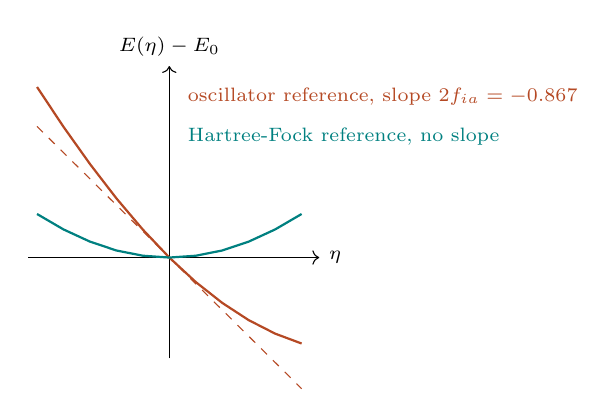
\begin{tikzpicture}[scale=1,x=14cm,y=16cm]
    \draw[->] (-0.16,0) -- (0.17,0) node[right,dlab] {$\eta$};
    \draw[->] (0,-0.10) -- (0,0.19) node[above,dlab] {$E(\eta)-E_0$};
    \draw[warm,thick] plot coordinates {(-0.150,0.1692) (-0.120,0.1297) (-0.090,0.0928) (-0.060,0.0587) (-0.030,0.0277) (0.000,0.0000) (0.030,-0.0243) (0.060,-0.0450) (0.090,-0.0621) (0.120,-0.0755) (0.150,-0.0853)};
    \draw[warm,dashed] (-0.15,0.1301) -- (0.15,-0.1301);
    \draw[teal,thick] plot coordinates {(-0.150,0.0432) (-0.120,0.0279) (-0.090,0.0158) (-0.060,0.0070) (-0.030,0.0018) (0.000,0.0000) (0.030,0.0018) (0.060,0.0070) (0.090,0.0158) (0.120,0.0279) (0.150,0.0432)};
    \node[dlab,warm,anchor=west] at (0.01,0.16) {oscillator reference, slope $2f_{ia}=-0.867$};
    \node[dlab,teal,anchor=west] at (0.01,0.12) {Hartree-Fock reference, no slope};
  \end{tikzpicture}
  \end{center}
  \scriptsize $E(\eta)-E_0$ for real $\eta$ and the pair $(a,i)=(4,2)$: a line through $E_0$ bent by the quadratic term, and a parabola with its minimum at $\eta=0$.
  \end{columns}
\end{frame}

\begin{frame}{The general variation, and what is still missing}
  \footnotesize
  A general first-order variation of the determinant is a superposition of the single ones,
  \[
    \ket{\Phi'_0}=\ket{\Phi_0}+\sum_{a>F}\sum_{i\le F}\eta_{ai}\,a_a^{\dagger}a_i\ket{\Phi_0}+\bigO(\eta^2),
  \]
  and since the $1p$-$1h$ determinants are mutually orthogonal and orthogonal to $\ket{\Phi_0}$, stationarity under it is stationarity under each term separately: $\element{a}{\hat{f}}{i}=0$ for every pair is the \alert{complete} first-order condition.
  \begin{block}{Two questions, both needing second order}
    \begin{enumerate}
      \item Are the $1p$-$1h$ excitations really all there is -- does the family of determinants near $\ket{\Phi_0}$ have exactly $(n-N)\times N$ complex parameters, and no others?
      \item Is the stationary point a minimum?
    \end{enumerate}
  \end{block}
  Answering them means writing down the \emph{exact} form of an arbitrary nearby determinant, not merely its first-order approximation. That is Thouless' theorem -- Friday.
  \vspace{0.3em}
  \mbbox{Three derivations of one equation: coefficients with multipliers give $\bm{h}^{\mathrm{HF}}\bm{C}=\bm{\epsilon}\bm{C}$; one orbital at a time gives $f_{ai}=0$; the determinant as a whole will give $f_{ai}=0$ plus the stability matrix.}
\end{frame}

% ======================================================================
\section{Friday, lecture 3: Thouless' theorem}
% ======================================================================

\begin{frame}{Where Thursday ended, and what a nearby determinant is}
  \footnotesize
  \begin{itemize}
    \item The ansatz: $\ket{\Phi_0}=\ket{c}=a_i^{\dagger}a_j^{\dagger}\cdots a_l^{\dagger}\ket{0}$, and we seek the determinant for which $E_0=\element{c}{\hat{H}}{c}$ is a local minimum.
    \item Stationarity: $\element{\delta c}{\hat{H}}{c}=0$ for every \emph{admissible} $\ket{\delta c}$ -- every variation that keeps $\ket{c}+\ket{\delta c}$ a Slater determinant. Thursday used $\ket{\delta c}=\eta\,a_a^{\dagger}a_i\ket{c}$ to first order. To go further we need to know what the neighbourhood of a determinant looks like \emph{inside the set of determinants}.
  \end{itemize}
  \begin{block}{Theorem (Thouless, 1960)}
    Any Slater determinant $\ket{c'}$ that is not orthogonal to a given determinant $\ket{c}=\prod_{i\le F}a_i^{\dagger}\ket{0}$ can be written as
    \[
      \ket{c'}=\exp\Bigl\{\sum_{a>F}\sum_{i\le F}C_{ai}\,a_a^{\dagger}a_i\Bigr\}\ket{c}=e^{\hat{T}}\ket{c}.
    \]
  \end{block}
  In words: every determinant in the neighbourhood of $\ket{c}$ is obtained from it by an exponentiated linear combination of $1p$-$1h$ excitations. The manifold of Slater determinants is parametrised, near any point, by the $(n-N)\times N$ complex amplitudes $C_{ai}$ \alert{and by nothing else} -- so the Hartree-Fock variation has exactly that many degrees of freedom, and the $2p$-$2h$, $3p$-$3h$, \dots\ admixtures that a general state has are all generated by the exponential.
  \vspace{0.3em}
  The proof has three steps: the exponential collapses; the result is a determinant; every determinant is of this form.
\end{frame}

\begin{frame}{Step one: the exponential collapses}
  \footnotesize
  The exponential of a sum factorises into a product of exponentials only when the operators commute (otherwise Baker-Campbell-Hausdorff, section 6.8, supplies the correction). Here we are lucky. For $a,b>F$ and $i,j\le F$ the index sets are disjoint, so $a_ia_b^{\dagger}=-a_b^{\dagger}a_i$ and $a_ja_a^{\dagger}=-a_a^{\dagger}a_j$, and both orderings reduce to $-a_a^{\dagger}a_b^{\dagger}a_ia_j$:
  \[
    \bigl[a_a^{\dagger}a_i,\;a_b^{\dagger}a_j\bigr]=0 .
  \]
  Write $\hat{T}=\sum_{i\le F}\hat{T}_i$ with $\hat{T}_i=\sum_{a>F}C_{ai}a_a^{\dagger}a_i$. Then $e^{\hat{T}}=\prod_ie^{\hat{T}_i}$, and each factor truncates, because
  \[
    \hat{T}_i^2=\sum_{ab>F}C_{ai}C_{bi}\,a_a^{\dagger}a_i\,a_b^{\dagger}a_i=0
  \]
  -- the rightmost $a_i$ empties hole $i$ and the second one annihilates the state ($a_i^2=0$). Hence
  \begin{block}{}
    \[
      \ket{c'}=\prod_{i\le F}\Bigl\{1+\sum_{a>F}C_{ai}\,a_a^{\dagger}a_i\Bigr\}\ket{c}.
    \]
  \end{block}
  \alert{This is not $1+\hat{T}$.} The cross terms $\hat{T}_i\hat{T}_j$, $i\ne j$, survive and are $2p$-$2h$ admixtures; $\hat{T}_i\hat{T}_j\hat{T}_k$ are $3p$-$3h$, and so on up to $Np$-$Nh$. They are second and higher order in the amplitudes, which is why dropping them is legitimate for an \emph{infinitesimal} variation -- exactly what Thursday did, and what the stability analysis will do at the next order.
\end{frame}

\begin{frame}{Step two: the product is a single determinant}
  \footnotesize
  Insert $\ket{c}=a_{i_1}^{\dagger}a_{i_2}^{\dagger}\cdots a_{i_N}^{\dagger}\ket{0}$. The factor labelled $i_1$ acts only on $a_{i_1}^{\dagger}$ (it commutes with every other creation operator and annihilates the vacuum), the factor labelled $i_2$ only on $a_{i_2}^{\dagger}$, and so on:
  \begin{align*}
    \ket{c'}&=\Bigl(1+\sum_{a}C_{ai_1}a_a^{\dagger}a_{i_1}\Bigr)a_{i_1}^{\dagger}\Bigl(1+\sum_aC_{ai_2}a_a^{\dagger}a_{i_2}\Bigr)a_{i_2}^{\dagger}\cdots\ket{0}
    =\prod_{i\le F}\Bigl(a_i^{\dagger}+\sum_{a>F}C_{ai}a_a^{\dagger}\Bigr)\ket{0}.
  \end{align*}
  \begin{block}{New creation operators}
    \[
      b_i^{\dagger}=a_i^{\dagger}+\sum_{a>F}C_{ai}a_a^{\dagger},\qquad\ket{c'}=\prod_{i\le F}b_i^{\dagger}\ket{0}.
    \]
  \end{block}
  \begin{itemize}
    \item $\ket{c'}$ has exactly the form of a Slater determinant: \alert{the rotated state is a single determinant, not a superposition}. This is the whole point.
    \item The new orbitals $\psi_i=\phi_i+\sum_aC_{ai}\phi_a$ are Thursday's variation for all $(i,a)$ at once -- with the exponential supplying, automatically, the products that make the result an exact determinant instead of a first-order approximation.
    \item They are not normalised ($\braket{\psi_i}{\psi_j}=\delta_{ij}+\sum_aC_{ai}^{*}C_{aj}$) and $\braket{c}{c'}=1$: this is \emph{intermediate normalisation}, the same convention as for the FCI amplitudes of week 38. A unitary mixing of the $b_i^{\dagger}$ changes the determinant by a factor only (section 6.3), so nothing is lost.
  \end{itemize}
\end{frame}

\begin{frame}[shrink=2]{Step three: it is the general determinant}
  \scriptsize
  $b_i^{\dagger}$ looks less general than it should, because the sum runs only over $a>F$. Take the most general new orbitals,
  \[
    \tilde{b}_i^{\dagger}=\sum_pf_{ip}\,a_p^{\dagger},\qquad\ket{\tilde{c}}=\prod_{i\le F}\tilde{b}_i^{\dagger}\ket{0},
  \]
  with $f$ unitary, and require only $\braket{c}{\tilde{c}}\ne0$. The overlap is
  \[
    \braket{c}{\tilde{c}}=\bra{0}a_{i_N}\cdots a_{i_1}\Bigl(\sum_pf_{i_1p}a_p^{\dagger}\Bigr)\cdots\Bigl(\sum_tf_{i_Nt}a_t^{\dagger}\Bigr)\ket{0}=\det\bigl(f_{ip}\bigr)_{i,p\le F},
  \]
  the determinant of the \emph{occupied block} of $f$: only terms with all $p\le F$ survive the vacuum expectation value, and the sum over permutations reconstructs a determinant.
  \begin{itemize}
    \item The hypothesis $\braket{c}{\tilde{c}}\ne0$ says exactly that the occupied block is invertible, and intermediate normalisation rescales it to $\det(f_{ip})=1$. With $f^{-1}$ (of the occupied block) available,
    \[
      \sum_{i\le F}f^{-1}_{ki}\tilde{b}_i^{\dagger}=\sum_i\sum_pf^{-1}_{ki}f_{ip}a_p^{\dagger}
      =a_k^{\dagger}+\sum_{p>F}\Bigl(\sum_{i\le F}f^{-1}_{ki}f_{ip}\Bigr)a_p^{\dagger},
    \]
    the terms with $p\le F$ having collapsed to $\delta_{kp}$. Setting $C_{pk}=\sum_if^{-1}_{ki}f_{ip}$ returns $b_k^{\dagger}$ exactly.
    \item A unitary (here: invertible) mixing of the $\tilde{b}^{\dagger}$ changes the determinant only by a factor, so $\ket{\tilde{c}}$ and $\ket{c'}$ are the same state. \alert{The theorem is proved.}
  \end{itemize}
  \begin{block}{What the hypothesis excludes}\scriptsize
    Determinants orthogonal to $\ket{c}$ -- e.g.\ $\ket{\Phi_i^a}$ itself -- cannot be reached by $e^{\hat{T}}\ket{c}$, whose overlap with $\ket{c}$ is always one. They are ``infinitely far away'' in the amplitudes: $C_{ai}\to\infty$. For a local variation this is no restriction at all.
  \end{block}
\end{frame}

\begin{frame}{Numerical check}
  \footnotesize
  \texttt{hartreefock.py}, class \texttt{ThoulessRotation}: six orbitals, three particles, random amplitudes $C_{ai}$ of size $0.3$, everything in the $\binom63=20$-dimensional determinant space of week 38.
  \begin{center}\scriptsize
  \renewcommand{\arraystretch}{1.1}
  \begin{tabular}{lr}\toprule
  $\max|[\hat{T}_i,\hat{T}_j]|$ & $2.8\times10^{-17}$\\
  $\max|\hat{T}_i^2|$ & $0$\\
  $\bigl|e^{\hat{T}}\ket{c}-\prod_ib_i^{\dagger}\ket{0}\bigr|$ & $5.6\times10^{-17}$\\
  $\braket{c}{e^{\hat{T}}c}$ & $1.000000000000$\\
  $\det$ of the occupied block of the orbital matrix & $1.000000000000$\\\bottomrule
  \end{tabular}
  \qquad
  \begin{tabular}{rrr}\toprule
  scale $s$ & $\bigl|e^{s\hat{T}}\ket{c}-(1+s\hat{T})\ket{c}\bigr|$ & ratio\\\midrule
  $0.4$ & $3.68\times10^{-2}$ & \\
  $0.2$ & $9.20\times10^{-3}$ & $4.00$\\
  $0.1$ & $2.30\times10^{-3}$ & $4.00$\\
  $0.05$ & $5.75\times10^{-4}$ & $4.00$\\
  $0.025$ & $1.44\times10^{-4}$ & $4.00$\\\bottomrule
  \end{tabular}
  \end{center}
  \begin{itemize}
    \item The rotated state is a determinant to machine precision, and its overlap with the reference is exactly one -- it is never orthogonal to the state we started from: exactly the freedom Hartree-Fock explores.
    \item Halving the amplitudes divides the discarded piece $e^{\hat{T}}-(1+\hat{T})$ by four: the $2p$-$2h$ admixtures are second order, as claimed. The notebook repeats this with the self-contained bit code of week 38.
  \end{itemize}
\end{frame}

\begin{frame}{Pause to think: counting, and what the exponential does}
  \thinkq{3}{
  \begin{enumerate}
    \item Eight orbitals, four particles. How many complex parameters does Thouless' theorem give the neighbourhood of a determinant? How many does a general normalised state in the $70$-dimensional space have? Where did the rest go?
    \item Write out $e^{\hat{T}}\ket{c}$ for $N=2$ explicitly. Which determinants appear, with which amplitudes? What does this say about the coupled-cluster ansatz $e^{\hat{T}_1}\ket{c}$ of chapter 10, and about why CIS gives nothing in a Hartree-Fock basis?
  \end{enumerate}}
\end{frame}

\begin{frame}{Answer}
  \thinka{
  \begin{enumerate}
    \item $(n-N)\times N=16$ complex amplitudes $C_{ai}$, against $69$ for a general normalised state in $70$ dimensions. The other $53$ directions leave the manifold of determinants: $2p$-$2h$, $3p$-$3h$, $4p$-$4h$ amplitudes that are \emph{not} products of $1p$-$1h$ ones. Hartree-Fock optimises $16$ parameters of a $69$-parameter problem; correlation is the other $53$.
    \item $e^{\hat{T}}\ket{c}=(1+\hat{T}_1)(1+\hat{T}_2)\ket{c}=\ket{c}+\sum_aC_{a1}\ket{\Phi_1^a}+\sum_bC_{b2}\ket{\Phi_2^b}+\sum_{ab}C_{a1}C_{b2}\,a_a^{\dagger}a_1a_b^{\dagger}a_2\ket{c}$. The doubles appear with amplitudes that are \emph{products} of singles amplitudes, $C_{12}^{ab}=C_{a1}C_{b2}-C_{b1}C_{a2}$: no freedom of their own. So $e^{\hat{T}_1}\ket{c}$ is just another determinant (Thouless), coupled cluster with singles only can never beat Hartree-Fock, $\hat{T}_2$ is the first correlating operator, and in a Hartree-Fock basis ($f_{ai}=0$) the singles amplitudes start at second order. CIS returns $E^{\mathrm{HF}}$ for the same reason: the singles span the tangent space of the determinant manifold at its stationary point.
  \end{enumerate}}
\end{frame}

\begin{frame}{What Thouless' theorem buys us}
  \footnotesize
  Any nearby determinant is
  \[
    \ket{c'}=\ket{c}+\ket{\delta c},\qquad\ket{c'}\simeq\Bigl(1+\sum_{ai}\delta C_{ai}\,a_a^{\dagger}a_i\Bigr)\ket{c}\quad\text{to first order},
  \]
  and the stationarity condition $\element{\delta c}{\hat{H}}{c}=0$ becomes
  \[
    \sum_{ai}\delta C_{ai}^{*}\,\element{c}{a_i^{\dagger}a_a\hat{H}}{c}=0\ \text{ for arbitrary }\delta C
    \qquad\Longrightarrow\qquad
    \element{\Phi_i^a}{\hat{H}}{\Phi_0}=f_{ai}=0 ,
  \]
  Thursday's condition for all pairs at once, and Brillouin's theorem.
  \begin{itemize}
    \item Thouless' theorem confirms what Thursday assumed: to first order the $1p$-$1h$ excitations \emph{exhaust} the neighbourhood of a determinant, so the single-orbital variations were the general case.
    \item Three derivations, one equation. What the third route adds is the \alert{exact} form of the neighbourhood -- and with it the ability to go to second order, which is the subject of the next lecture.
  \end{itemize}
  \mbbox{The Thouless rotation is also how mean fields are \emph{parametrised} in practice: the Lipkin model below rotates every orbital by the same angle, $C_{ai}=\tan(\alpha/2)\,\delta_{pq}$; deformed nuclei, symmetry-broken Hartree-Fock for Hubbard, and the BCS state of chapter 7 are all Thouless rotations of a symmetric reference. The unitary form $e^{\hat{T}-\hat{T}^{\dagger}}$ is the orbital-rotation step of every modern Hartree-Fock code.}
\end{frame}

% ======================================================================
\section{Friday, lecture 4: Stability of the Hartree-Fock solution}
% ======================================================================

\begin{frame}[shrink=4]{Stationary is not minimal (section 6.10)}
  \footnotesize
  The variational condition $f_{ai}=0$ guarantees only that $\element{c}{\hat{H}}{c}$ is \emph{stationary}. A stationary point may be a minimum, a maximum or a saddle -- and it matters:
  \begin{itemize}
    \item a Hartree-Fock solution on a saddle is a poor reference for perturbation theory or coupled cluster, because the corrections it generates are organised about the wrong state;
    \item there is a direction in the space of determinants along which the energy \emph{decreases}, so a better single determinant exists -- usually one that breaks a symmetry of $\hat{H}$ which the reference respected.
  \end{itemize}
  \begin{block}{The question}
    Is
    \[
      \frac{\element{c'}{\hat{H}}{c'}}{\braket{c'}{c'}}\ \ge\ \element{c}{\hat{H}}{c}=E_0
    \]
    for \emph{every} nearby determinant $\ket{c'}=\ket{c}+\ket{\delta c}$?
  \end{block}
  Thouless' theorem tells us what ``every nearby determinant'' means, and lets us expand to second order:
  \[
    \ket{c'}=e^{\sum\delta C_{ai}a_a^{\dagger}a_i}\ket{c}
    =\Bigl\{1+\sum_{ai}\delta C_{ai}a_a^{\dagger}a_i+\frac{1}{2!}\sum_{abij}\delta C_{ai}\delta C_{bj}\,a_a^{\dagger}a_ia_b^{\dagger}a_j+\cdots\Bigr\}\ket{c},
  \]
  \vspace{-0.8em}
  \[
    \braket{c'}{c'}=1+\sum_{ai}|\delta C_{ai}|^2+\bigO(\delta C^3)
  \]
  (intermediate normalisation $\braket{c'}{c}=1$; the cross terms between $1$ and the linear piece vanish since $\element{c}{a_a^{\dagger}a_i}{c}=0$, and the linear piece with itself gives the sum of squares because the $1p$-$1h$ states are orthonormal).
\end{frame}

\begin{frame}{The energy to second order}
  \footnotesize
  Expand the numerator and use $f_{ai}=0$ to kill the terms linear in $\delta C$:
  \begin{align*}
    \element{c'}{\hat{H}}{c'}
    &=\element{c}{\hat{H}}{c}
    +\sum_{ab>F}\sum_{ij\le F}\delta C_{ai}^{*}\delta C_{bj}\,\element{c}{a_i^{\dagger}a_a\,\hat{H}\,a_b^{\dagger}a_j}{c}\\
    &\quad+\frac{1}{2!}\sum\delta C_{ai}\delta C_{bj}\,\element{c}{\hat{H}\,a_a^{\dagger}a_ia_b^{\dagger}a_j}{c}
    +\frac{1}{2!}\sum\delta C_{ai}^{*}\delta C_{bj}^{*}\,\element{c}{a_j^{\dagger}a_ba_i^{\dagger}a_a\,\hat{H}}{c}+\cdots
  \end{align*}
  Each expectation value is a Wick calculation of week 37. With $\hat{H}=\sum_{pq}\element{p}{\hat{h}_0}{q}a_p^{\dagger}a_q+\frac14\sum\element{pq}{\hat{v}}{rs}a_p^{\dagger}a_q^{\dagger}a_sa_r$:
  \begin{itemize}
    \item \textbf{First line} ($1p$-$1h$ to $1p$-$1h$, the matrix element of week 38's CI matrix): collecting the surviving contractions in a Hartree-Fock basis,
    \[
      E_0\sum_{ai}|\delta C_{ai}|^2+\sum_{ai}|\delta C_{ai}|^2\bigl(\varepsilon_a-\varepsilon_i\bigr)-\sum_{ijab}\element{aj}{\hat{v}}{bi}\,\delta C_{ai}^{*}\delta C_{bj} .
    \]
    The first term is $E_0$ times the norm correction; the second is the unperturbed excitation energy; the third is the particle-hole interaction.
    \item \textbf{Second line} (reference to $2p$-$2h$): only $\hat{V}_N$ contributes,
    \[
      \frac12\sum_{ijab}\element{ab}{\hat{v}}{ij}\,\delta C_{ai}^{*}\delta C_{bj}^{*}
      \qquad\text{(and the third line is its Hermitian conjugate).}
    \]
  \end{itemize}
\end{frame}

\begin{frame}{The stability matrix}
  \footnotesize
  Define the two antisymmetrised blocks and the diagonal matrix of excitation energies,
  \[
    A_{ai,bj}=-\element{aj}{\hat{v}}{bi}_{\mathrm{AS}},\qquad
    B_{ai,bj}=\element{ab}{\hat{v}}{ij}_{\mathrm{AS}},\qquad
    \Delta_{ai,bj}=(\varepsilon_a-\varepsilon_i)\,\delta_{ab}\delta_{ij}.
  \]
  Then, dividing by the norm $1+\sum|\delta C|^2$,
  \begin{block}{}
    \[
      \frac{\element{c'}{\hat{H}}{c'}}{\braket{c'}{c'}}=E_0+\frac{\Delta E}{1+\sum_{ai}|\delta C_{ai}|^2},
      \qquad
      \Delta E=\frac12\bra{\chi}\hat{M}\ket{\chi},
      \qquad
      \chi=\begin{bmatrix}\delta C\\ \delta C^{*}\end{bmatrix},\quad
      \hat{M}=\begin{pmatrix}\Delta+A & B\\ B^{*} & \Delta+A^{*}\end{pmatrix}.
    \]
  \end{block}
  \begin{itemize}
    \item The denominator is positive, so \alert{the Hartree-Fock solution is a local minimum if and only if $\Delta E=\frac12\bra{\chi}\hat{M}\ket{\chi}\ge0$ for every $\chi$}, i.e.\ if and only if every eigenvalue of $\hat{M}$ is non-negative.
    \item A necessary (not sufficient) condition, from $\chi$ restricted to the upper block: $\Delta+A\ge0$ as a matrix. Cheap, and the usual first check.
    \item Why does $\chi$ contain both $\delta C$ and $\delta C^{*}$? Because the second-order energy has terms $\delta C^{*}\delta C$ (the $A$ block), $\delta C\,\delta C$ and $\delta C^{*}\delta C^{*}$ (the $B$ blocks): a quadratic form in the \emph{real} variables $\mathrm{Re}\,\delta C$, $\mathrm{Im}\,\delta C$, written compactly in the complex ones. Thursday's one-parameter family is the $1\times1$ case, with $B_{ai,ai}=\element{aa}{\hat{v}}{ii}=0$ by antisymmetry.
  \end{itemize}
\end{frame}

\begin{frame}{The stability matrix is the RPA matrix}
  \small
  \mbbox{$\Delta+A$ is exactly the Hamiltonian restricted to the $1p$-$1h$ space, measured from $E_0$: the matrix of the Tamm-Dancoff approximation and of CIS. The full $\hat{M}$, with its $B$ blocks, is the matrix of the random-phase approximation (chapter 7). So ``the Hartree-Fock solution is stable'' and ``the RPA frequencies are real'' are one and the same statement, and an imaginary RPA frequency is not a numerical accident but a signal that the mean field itself is wrong. TDA and RPA are the second derivative of the Hartree-Fock energy surface.}
  \vspace{0.4em}
  \begin{itemize}
    \item In practice: solve the Hartree-Fock equations, then diagonalise $\Delta+A$ (cheap, necessary) and, if in doubt, $\hat{M}$ (sufficient). A negative eigenvalue names the \emph{direction} $\chi$ in which to deform the reference -- which is how symmetry-broken solutions are found.
    \item Two examples follow: one where $\hat{M}$ goes negative at a critical coupling (Lipkin), and one where it never does but the mean field is nevertheless useless (pairing).
  \end{itemize}
\end{frame}

\begin{frame}{An explicit instability: the Lipkin model (section 6.11)}
  \footnotesize
  $N$ particles in two $N$-fold degenerate levels separated by $\varepsilon$, $W=0$:
  \[
    \hat{H}=\varepsilon\hat{J}_z+\frac{V}{2}\bigl(\hat{J}_+^2+\hat{J}_-^2\bigr),
    \qquad
    \hat{J}_z=\tfrac12\sum_p\bigl(a_{p+}^{\dagger}a_{p+}-a_{p-}^{\dagger}a_{p-}\bigr),\quad
    \hat{J}_+=\sum_pa_{p+}^{\dagger}a_{p-}.
  \]
  The natural mean field rotates every single-particle state by the same angle in the two-level space -- a Thouless rotation with $C_{ai}=\tan(\alpha/2)\,\delta_{pq}$, normalised:
  \[
    b_p^{\dagger}=\cos\tfrac{\alpha}{2}\,a_{p-}^{\dagger}+\sin\tfrac{\alpha}{2}\,a_{p+}^{\dagger},
    \qquad
    \boxed{\;\frac{E(\alpha)}{N}=-\frac{\varepsilon}{2}\cos\alpha-\frac{\varepsilon\chi}{4}\sin^2\alpha,\qquad\chi=\frac{|V|(N-1)}{\varepsilon}\;}
  \]
  \begin{itemize}
    \item $\frac1N\frac{\dd E}{\dd\alpha}=\frac{\varepsilon}{2}\sin\alpha\,(1-\chi\cos\alpha)$: two stationary points, the \emph{spherical} solution $\alpha=0$ (always) and a \emph{deformed} solution $\cos\alpha=1/\chi$ (only for $\chi\ge1$).
    \item $\frac1N\frac{\dd^2E}{\dd\alpha^2}\big|_{\alpha=0}=\frac{\varepsilon}{2}(1-\chi)$ changes sign at $\chi=1$: the spherical solution turns from a minimum into a maximum exactly where the deformed one appears -- a continuous symmetry-breaking transition.
    \item At $\alpha=0$ the energy is $-\varepsilon/2$ per particle for \emph{every} coupling: the interaction changes $J_z$ by two units and has no expectation value in the undeformed determinant. \alert{What changes with $\chi$ is the curvature, not the energy} -- and no energy criterion would notice.
    \item The deformed minima come in pairs $\pm\alpha$ (the mean field has broken a symmetry of $\hat{H}$) and their energy is $-\frac{\varepsilon}{4}(\chi+1/\chi)$ per particle: at $\chi=1.5$ only $0.042\varepsilon$ below the spherical state.
  \end{itemize}
\end{frame}

\begin{frame}{The Lipkin energy surface}
  \begin{columns}[T]
    \column{0.6\textwidth}
    
\includegraphics[width=\textwidth]{chapter06/hf_fig02}
    \column{0.4\textwidth}
    \footnotesize
    $E(\alpha)/N$ against the rotation angle, $N=4$, $\varepsilon=1$, $W=0$.
    \begin{itemize}
      \item All curves pass through $-\varepsilon/2$ at $\alpha=0$.
      \item $\chi=0.5$: a simple well.
      \item $\chi=1$: the curvature has vanished, the surface is quartic at the origin.
      \item $\chi=1.5$, $2.5$: $\alpha=0$ is a local maximum, with two degenerate deformed minima at $\alpha=\pm0.841$ and $\pm1.159$, energies $-0.542$ and $-0.725$.
    \end{itemize}
    Almost everything the stability analysis does algebraically can be read off this picture. The next slide does it algebraically anyway, because for a realistic system there is no $\alpha$ to plot against.
  \end{columns}
\end{frame}

\begin{frame}{The stability matrix says the same, without the parametrisation}
  \scriptsize
  \begin{columns}[T]
    \column{0.48\textwidth}
    \begin{itemize}
      \item The interaction changes $J_z$ by two units, so it has no matrix element within the $1p$-$1h$ space: $A=0$ and $\Delta+A=\varepsilon\bm{1}$.
      \item $B$ has elements $\pm V$ connecting different pairs (a pair $p$ raised and a pair $q$ raised is the $2p$-$2h$ state $\hat{J}_+^2$ makes); its largest eigenvalue is $|V|(N-1)$.
      \item Hence
      \[
        \boxed{\;\lambda_{\min}(\hat{M})=\varepsilon-|V|(N-1)=\varepsilon(1-\chi)\;}
      \]
      which is the second derivative of the previous slide up to the factor $N/2$.
    \end{itemize}
    \texttt{hartreefock.py} builds $\hat{M}$ numerically from $\hat{H}$ in the determinant basis ($N=4$, $\varepsilon=1$):
    \begin{center}\tiny
    \renewcommand{\arraystretch}{1.05}
    \setlength{\tabcolsep}{3pt}
    \begin{tabular}{rrrrrl}\toprule
    $\chi$ & $\lambda_{\min}(\hat{M})$ & $\alpha_{\min}$ & $E_{\mathrm{mf}}$ & $E_{\mathrm{exact}}$ & solution\\\midrule
    $0.25$ & $0.75$ & $0$ & $-2.000000$ & $-2.020726$ & spherical\\
    $0.50$ & $0.50$ & $0$ & $-2.000000$ & $-2.081666$ & spherical\\
    $0.90$ & $0.10$ & $0$ & $-2.000000$ & $-2.253886$ & spherical\\
    $1.00$ & $0.00$ & $0$ & $-2.000000$ & $-2.309401$ & critical\\
    $1.50$ & $-0.50$ & $0.841$ & $-2.166667$ & $-2.645751$ & deformed\\
    $2.00$ & $-1.00$ & $1.047$ & $-2.500000$ & $-3.055050$ & deformed\\\bottomrule
    \end{tabular}
    \end{center}
    \column{0.52\textwidth}
    
\includegraphics[width=\textwidth]{chapter06/hf_fig03}
    \scriptsize The numerical eigenvalues sit on the line $\varepsilon(1-\chi)$ over the whole range and keep falling beyond the transition: a negative eigenvalue is a direction along which the energy decreases without limit until the nonlinearity of the parametrisation catches it.
  \end{columns}
\end{frame}

\begin{frame}{Pause to think: stable, and useless}
  \thinkq{4}{
  \begin{enumerate}
    \item For $\chi=2$ the spherical Lipkin determinant satisfies $f_{ai}=0$ exactly and obeys Brillouin's theorem. Is it a Hartree-Fock solution? What goes wrong if one builds second-order perturbation theory on it?
    \item The pairing model of weeks 37--38 (four doubly degenerate levels, four particles, $\varepsilon_p=p-1$, pairing strength $g$): last week we saw that Hartree-Fock does nothing for it. Is the reference \emph{stable}? Guess $\lambda_{\min}(\hat{M})$ as a function of $g$ before looking at the next slide. Hint: which $1p$-$1h$ pairs does $B$ connect, and what is $\Delta$ for them?
  \end{enumerate}}
\end{frame}

\begin{frame}{Answer}
  \thinka{
  \begin{enumerate}
    \item It is a genuine stationary point of the energy on the manifold of determinants, so it satisfies the Hartree-Fock \emph{equations} -- but it is a saddle, not a minimum, and a local minimum is what the variational principle asked for. Second-order perturbation theory about it has the form $\sum|\element{\Phi_{ij}^{ab}}{\hat{V}}{\Phi_0}|^2/(E_0-E_{ij}^{ab})$; in the unstable channel the relevant ``excitation energy'' is governed by $\lambda_{\min}<0$, the denominators are small and of the wrong sign, and the series is organised about the wrong state. The deformed solution is $0.5$ lower at $\chi=2$, but still $0.55$ above the exact answer, and has broken a symmetry that must eventually be restored.
  \end{enumerate}}
\end{frame}

\begin{frame}{Answer, continued}
  \thinka{
  \begin{enumerate}\setcounter{enumi}{1}
    \item $A=0$: the pairing interaction cannot scatter a single particle-hole pair, so $\Delta+A$ is diagonal with $\Delta=\varepsilon_q-\varepsilon_p+g/2$ for the pair $p\to q$ (breaking the pair at $p$ costs its pairing energy; $\lambda_{\min}(\Delta+A)=1+g/2$, so the necessary condition holds). $B$ couples $\delta C_{q\uparrow,p\uparrow}$ to $\delta C^{*}_{q\downarrow,p\downarrow}$ through $\element{q\!\uparrow q\!\downarrow}{\hat{v}}{p\!\uparrow p\!\downarrow}=-g/2$, so $\hat{M}$ falls apart into $2\times2$ blocks $\begin{pmatrix}\Delta & -g/2\\ -g/2 & \Delta\end{pmatrix}$ with eigenvalues $\varepsilon_q-\varepsilon_p$ and $\varepsilon_q-\varepsilon_p+g$: moving the pair \emph{coherently} costs exactly the level spacing, the interaction cancels out, and $\lambda_{\min}(\hat{M})=\varepsilon_3-\varepsilon_2=1$ \emph{for every} $g$ (numerically $1.0000$ at $g=0.25,\dots,3$). The reference is stable, and Hartree-Fock -- any number-conserving mean field -- can never capture pair correlations. The mean field that does is the BCS state of chapter 7, a Thouless-like rotation that breaks particle-number symmetry instead.
  \end{enumerate}}
\end{frame}

\begin{frame}{Two lessons, and where this goes}
  \small
  \begin{block}{Lesson 1: satisfying the Hartree-Fock equations is not enough}
    A solution can satisfy $f_{ai}=0$ perfectly, obey Brillouin's theorem, and be a saddle. Only the stability matrix -- equivalently, the RPA frequencies -- tells the difference, and one needs the criterion, not a plausibility argument: at $\chi=1.5$ the deformed state is a mere $0.042\varepsilon$ per particle below the spherical one.
  \end{block}
  \begin{block}{Lesson 2: symmetry breaking is a device, and the bill comes later}
    The deformed solution buys a lower energy by breaking a symmetry the exact ground state does not break. It captures correlations cheaply -- and the symmetry must eventually be restored, by projection or by a method that never broke it. Deformed nuclei, spin-density waves in the Hubbard model and BCS superconductivity are all this mechanism.
  \end{block}
  \begin{itemize}
    \item Stable but useless (pairing model): the mean field is fine, the physics is in the doubles; perturbation theory and coupled cluster start there.
    \item Unstable (Lipkin, $\chi>1$; Hubbard beyond a critical $U$): the mean field itself must change before any correlation method makes sense.
    \item In both cases the diagnosis is the same object, $\hat{M}$, and its eigenvalue problem is chapter 7.
  \end{itemize}
\end{frame}

% ======================================================================
\section{Exercises: week 39, and answers for week 38}
% ======================================================================

\begin{frame}{Exercise session: week 39 (suggested set)}
  \footnotesize
  Three exercises, one per derivation of the week. Full answers to the parts taken from the chapter exercise sections are in the lecture notes; the new parts are answered on next week's slides.
  \begin{block}{Exercise 1: varying one orbital (section 6.6; new)}
    \begin{enumerate}
      \item[a)] Let $\delta\phi_i=\sum_\lambda d_\lambda\phi_\lambda$ be arbitrary. Show, using linearity of the determinant in row $i$, that the components with $\lambda\le F$ change $\Phi_0$ by at most a factor, and that the normalisation constant is $N_i^{-2}=1+\sum_{a>F}|d_a|^2$ once the occupied components are dropped.
      \item[b)] Derive $E(\eta)=E_0+2\,\mathrm{Re}(\eta f_{ia})+|\eta|^2(\element{\Phi_i^a}{\hat{H}}{\Phi_i^a}-E_0)+\bigO(|\eta|^3)$ from the exact expression with the denominator $1+|\eta|^2$, and show that the cubic term is $-2|\eta|^2\,\mathrm{Re}(\eta f_{ia})$. What does a real $\eta$ alone fail to fix?
      \item[c)] With $\hat{H}=E_{\mathrm{ref}}+\hat{F}_N+\hat{V}_N$ normal ordered with respect to $\ket{\Phi_0}$, show that $\element{\Phi_0}{\hat{V}_N}{\Phi_i^a}=0$ by writing $\hat{V}_N$ in its particle-hole form (week 37) and letting each term act on $\ket{\Phi_i^a}$, without Wick's theorem. Then show that $f_{ai}=0$ for all pairs makes $\bm{f}$ block diagonal, and that diagonalising the blocks does not change $\ket{\Phi_0}$.
      \item[d)] For the random $n=8$, $N=4$ Hamiltonian of the week-38 notebook, plot $E(\eta)$ for real $\eta\in[-0.15,0.15]$ and the pair with the largest $|f_{ia}|$, in the original basis and in the Hartree-Fock basis. Check that the odd part of $E(\eta)$ equals $2\eta f_{ia}$ up to the cubic term, and that a purely imaginary $\eta$ produces no linear change.
    \end{enumerate}
  \end{block}
\end{frame}

\begin{frame}{Exercise session: week 39 (continued)}
  \footnotesize
  \begin{block}{Exercise 2: single-particle energies and Thouless' theorem (chapter 6, exercises 2b--c and 3a, 3b, 3d)}
    \begin{enumerate}
      \item[a)] Show that $E^{\mathrm{HF}}\ne\sum_i\varepsilon_i^{\mathrm{HF}}$ and derive $E^{\mathrm{HF}}=\sum_{i\le F}\varepsilon_i^{\mathrm{HF}}-\frac12\sum_{ij\le F}\element{ij}{\hat{v}}{ij}$. Verify it numerically for the trap system ($N=4$) or the random Hamiltonian.
      \item[b)] Koopmans: compute the energy of the determinant with orbital $k$ removed, with the remaining orbitals frozen, and show that it is $E^{\mathrm{HF}}-\varepsilon_k^{\mathrm{HF}}$. Why is the corresponding statement for \emph{adding} a particle in orbital $a$ less accurate?
      \item[c)] Prove $[a_a^{\dagger}a_i,a_b^{\dagger}a_j]=0$ from the anticommutation relations, marking where the disjointness of the particle and hole index sets is used. Show $\hat{T}_i^2=0$ and hence $e^{\hat{T}}=\prod_i(1+\hat{T}_i)$; write out the $2p$-$2h$ content of $\hat{T}_i\hat{T}_j$.
      \item[d)] Show $\braket{c}{\tilde{c}}=\det(f_{ip})_{i,p\le F}$ for $\tilde{b}_i^{\dagger}=\sum_pf_{ip}a_p^{\dagger}$, first for $N=2$ explicitly, then in general, and explain why $\braket{c}{\tilde{c}}\ne0$ is exactly what the proof needs.
    \end{enumerate}
  \end{block}
\end{frame}

\begin{frame}{Exercise session: week 39 (continued)}
  \footnotesize
  \begin{block}{Exercise 3: stability (chapter 6, exercise 5a--c, plus the pairing model)}
    \begin{enumerate}
      \item[a)] Derive the norm $\braket{c'}{c'}=1+\sum_{ai}|\delta C_{ai}|^2+\bigO(\delta C^3)$ of the Thouless-rotated determinant, keeping track of which terms are second order.
      \item[b)] From the second-order energy, obtain $\Delta E=\frac12\bra{\chi}\hat{M}\ket{\chi}$ and the blocks $\Delta$, $A$, $B$. Why does $\chi$ contain both $\delta C$ and $\delta C^{*}$? Show that $\hat{M}$ is Hermitian and that restricting $\chi$ to its upper half gives the necessary condition $\Delta+A\ge0$.
      \item[c)] Lipkin model, $W=0$: show $A=0$, show that the largest eigenvalue of $B$ is $|V|(N-1)$, and recover $\lambda_{\min}(\hat{M})=\varepsilon(1-\chi)$.
      \item[d)] Pairing model, four levels, four particles: show analytically that $\hat{M}$ falls apart into $2\times2$ blocks with eigenvalues $\varepsilon_q-\varepsilon_p$ and $\varepsilon_q-\varepsilon_p+g$, so that $\lambda_{\min}(\hat{M})=1$ for every $g$, and confirm it with the notebook. What does this say about the prospects of a number-conserving mean field for pairing?
    \end{enumerate}
  \end{block}
\end{frame}

\begin{frame}{Answers to the week-38 exercises: 1, bit patterns}
  \footnotesize
  \begin{block}{1a) Five orbitals, bits $\alpha_0\dots\alpha_4$, $\alpha_0$ leftmost}
    \begin{itemize}
      \item $a_3^{\dagger}a_1\ket{01011}$: occupied $\{1,3,4\}$. $a_1$: no occupied state below $1$, phase $+$, gives $\ket{00011}$. Then $a_3^{\dagger}$ on a state in which $3$ is \emph{occupied}: \alert{zero} (Pauli).
      \item $a_0^{\dagger}a_4\ket{01101}$: occupied $\{1,2,4\}$. $a_4$: two occupied states below $4$, phase $(-1)^2=+$, gives $\ket{01100}$; $a_0^{\dagger}$: none below, phase $+$; result $+\ket{11100}$. ``Between'' rule: occupied states strictly between $0$ and $4$ are $\{1,2\}$, two of them, phase $+$. Same answer.
      \item $a_4^{\dagger}a_3^{\dagger}a_1a_0\ket{11010}$: occupied $\{0,1,3\}$. $a_0$ then $a_1$ (rightmost first) give $+\ket{00010}$; $a_3^{\dagger}$ on occupied $3$: \alert{zero}.
    \end{itemize}
    Two of the three vanish -- the lesson is to check occupancy before counting signs. (Replace $a_3^{\dagger}$ by $a_2^{\dagger}$ in the first: occupied $\{1,3,4\}\to\{3,4\}\to\{2,3,4\}$, no occupied state between $1$ and $2$, answer $+\ket{00111}$.)
  \end{block}
\end{frame}

\begin{frame}{Answers to the week-38 exercises: 1, continued}
  \footnotesize
  \begin{block}{1b) The phase of $a_j^{\dagger}a_i$}
    $a_i$ contributes $(-1)^{n_<(i)}$, $n_<(i)$ the number of occupied states below $i$; $a_j^{\dagger}$ then contributes $(-1)^{n'_<(j)}$ counted in the state \emph{after} the removal. For $i<j$: $n'_<(j)=n_<(j)-1$ and $n_<(j)=n_<(i)+1+n_{(i,j)}$ ($i$ itself and the $n_{(i,j)}$ occupied states strictly between), so the total exponent is $2n_<(i)+n_{(i,j)}$. For $j<i$: $n'_<(j)=n_<(j)$ and $n_<(i)=n_<(j)+n_{(j,i)}$ ($j$ is empty), exponent $2n_<(j)+n_{(j,i)}$. Either way $(-1)^{l}$ with $l$ the number of occupied states strictly between. The argument uses $i\ne j$ when it says that $j$ is empty after the removal and that $i$ lies on one side of $j$; for $i=j$ the operator is the number operator with phase $+1$.
  \end{block}
  \begin{block}{1c) Counting}
    $a_p^{\dagger}a_q^{\dagger}a_sa_r\ket{\Phi}\ne0$ needs $r\ne s$ both occupied -- $N(N-1)$ ordered pairs -- and then $p\ne q$ both empty in the state with $r,s$ removed: $(n-N+2)(n-N+1)$. Total $N(N-1)(n-N+2)(n-N+1)$: for $n=40$, $N=8$ that is $56\times1122=62\,832$ against $n^4=2\,560\,000$, i.e.\ $2.5\%$. \texttt{apply\_hamiltonian} on random patterns with $n=8$, $N=4$ finds $360=12\times30$ non-zero quadruples, as the formula says.
  \end{block}
\end{frame}

\begin{frame}{Answers to the week-38 exercises: 2, the FCI equation from the variational principle}
  \footnotesize
  \begin{block}{2a) Rayleigh quotient}
    With $C$ and $C^{*}$ independent, $\dfrac{\partial}{\partial C_K^{*}}\dfrac{\bm{C}^{\dagger}\bm{H}\bm{C}}{\bm{C}^{\dagger}\bm{C}}=\dfrac{(\bm{H}\bm{C})_K}{\bm{C}^{\dagger}\bm{C}}-\dfrac{\bm{C}^{\dagger}\bm{H}\bm{C}}{(\bm{C}^{\dagger}\bm{C})^2}C_K=\dfrac{(\bm{H}\bm{C}-E\bm{C})_K}{\bm{C}^{\dagger}\bm{C}}$, which vanishes for all $K$ iff $\bm{H}\bm{C}=E\bm{C}$: the stationary points are the eigenvectors and the stationary values the eigenvalues. With a multiplier, $\partial[\bm{C}^{\dagger}\bm{H}\bm{C}-\lambda(\bm{C}^{\dagger}\bm{C}-1)]/\partial C_K^{*}=0$ gives $\bm{H}\bm{C}=\lambda\bm{C}$, and contracting with $\bm{C}^{\dagger}$, $\lambda=\bm{C}^{\dagger}\bm{H}\bm{C}=E$.
  \end{block}
  \begin{block}{2b) Two levels, one pair}
    $\bm{H}=\begin{pmatrix}-g/2 & -g/2\\ -g/2 & 2\xi-g/2\end{pmatrix}$, $\det(\bm{H}-E\bm{1})=(E+g/2)(E-2\xi+g/2)-g^2/4=0$, so $E_\pm=\xi-\dfrac{g}{2}\pm\sqrt{\xi^2+\dfrac{g^2}{4}}$. Expanding the root, $E_-=-\dfrac{g}{2}-\dfrac{g^2}{8\xi}+\dfrac{g^4}{128\xi^3}-\cdots$. Second-order perturbation theory: $E_{\mathrm{ref}}=-g/2$ and $E^{(2)}=\dfrac{|\element{\Phi_1}{\hat{H}}{\Phi_0}|^2}{E_{\mathrm{ref}}-H_{11}}=\dfrac{g^2/4}{-2\xi}=-\dfrac{g^2}{8\xi}$: the expansion of the exact root reproduces it term by term, and the next term, $+g^4/128$, is fourth order (there is no third-order term for this $2\times2$ problem). At $\xi=g=1$: $E_-=-0.618034$, second order $-0.625$.
  \end{block}
\end{frame}

\begin{frame}{Answers to the week-38 exercises: 2, continued}
  \footnotesize
  \begin{block}{2c) Characteristic polynomials}
    For the $6\times6$ seniority-zero matrix at $g=1$ (basis $\ket{12},\ket{13},\ket{14},\ket{23},\ket{24},\ket{34}$, diagonal $1,3,5,5,7,9$, off-diagonal $-\frac12$ between pairs sharing a level),
    \[
      p(E)=E^6-30E^5+352E^4-2038E^3+5979E^2-7940E+3100,
    \]
    trace $=30$ and $\det=3100$ by hand, the rest with \texttt{numpy.poly}; its roots $0.635548,\ 2.935381,\ 5,\ 5,\ 7.208940,\ 9.220130$ agree with \texttt{eigh} to $10^{-13}$ (the double root $5$ is the pair $\ket{14}\pm\ket{23}$, which the interaction does not split). For the $70\times70$ matrix the coefficients span $55$ orders of magnitude (largest $9.6\times10^{54}$), the roots computed from the \emph{exact} coefficients are off by up to $13$, and a relative noise of $10^{-14}$ on the coefficients makes them garbage -- while the same noise on the matrix moves the eigenvalues by $10^{-13}$. The eigenvalue problem is well conditioned; the polynomial is not. This is why nobody solves $\det(\bm{H}-E\bm{1})=0$ beyond $3\times3$.
  \end{block}
\end{frame}

\begin{frame}{Answers to the week-38 exercises: 2, interlacing}
  \footnotesize
  \begin{block}{2d) Interlacing (Hylleraas-Undheim-MacDonald)}
    Diagonalising the leading $k\times k$ blocks in the order $\ket{12},\ket{13},\ket{14},\ket{23},\ket{24},\ket{34}$:
    \begin{center}\scriptsize
    \begin{tabular}{r|llllll}
    $k$ & $E_1^{(k)}$ & $E_2^{(k)}$ & $E_3^{(k)}$ & $E_4^{(k)}$ & $E_5^{(k)}$ & $E_6^{(k)}$\\\hline
    1 & 1 &&&&&\\
    2 & 0.881966 & 3.118034 &&&&\\
    3 & 0.794697 & 3.052662 & 5.152641 &&&\\
    4 & 0.708712 & 3.000000 & 5.000000 & 5.291288 &&\\
    5 & 0.648907 & 3.000000 & 5.000000 & 5.102196 & 7.248898 &\\
    6 & 0.635548 & 2.935381 & 5.000000 & 5.000000 & 7.208940 & 9.220130
    \end{tabular}
    \end{center}
    Every column decreases monotonically as $k$ grows and $E_m^{(k)}\ge E_m^{(k+1)}\ge\cdots\ge E_m$: the $m$-th Ritz value in a subspace is an upper bound on the $m$-th exact eigenvalue, not only the lowest. (Reading down a column also shows $E_m^{(k)}\le E_{m+1}^{(k+1)}$, the interlacing proper.)
  \end{block}
\end{frame}

\begin{frame}[shrink=4]{Answers to the week-38 exercises: 3, truncations and size consistency}
  \footnotesize
  \begin{block}{3a) CIS and CID for the pairing model}
    Restricting the $70\times70$ matrix to excitation levels $\le0,1,2,3,4$ gives dimensions $1,17,53,69,70$. CIS returns exactly $E_{\mathrm{ref}}$ because $\element{\Phi_0}{\hat{H}}{\Phi_i^a}=0$: a single excitation breaks a pair and changes the seniority, which the pairing Hamiltonian conserves (week 38, exercise 2c of chapter 5). The reference is decoupled from the whole singles block, remains an exact eigenvector of the truncated matrix, and is its lowest eigenvalue for the couplings considered. CID keeps the reference and the four $2p$-$2h$ seniority-zero states $\ket{13},\ket{14},\ket{23},\ket{24}$ (plus $2p$-$2h$ broken-pair states that decouple); it misses the $4p$-$4h$ state $\ket{34}$, which is why the CID column of the week-38 table lies above FCI.
  \end{block}
  \begin{block}{3b) Two non-interacting copies}
    Two two-level systems, one pair each, levels $0,\xi,0,\xi$, the interaction acting within a copy only:
    \begin{center}\scriptsize
    \begin{tabular}{rllll}
    $g$ & $2E(A)$ & $E(AB)_{\mathrm{FCI}}$ & $E(AB)_{\mathrm{CID}}$ & CID error\\\hline
    0.25 & $-0.26556444$ & $-0.26556444$ & $-0.26550480$ & $5.96\times10^{-5}$\\
    0.50 & $-0.56155281$ & $-0.56155281$ & $-0.56066017$ & $8.93\times10^{-4}$\\
    1.00 & $-1.23606798$ & $-1.23606798$ & $-1.22474487$ & $1.13\times10^{-2}$
    \end{tabular}
    \end{center}
    Full CI is additive to machine precision ($E(A)=\xi-g/2-\sqrt{\xi^2+g^2/4}$ from 2b); the CID error grows by an order of magnitude each time $g$ is doubled.
  \end{block}
\end{frame}

\begin{frame}{Answers to the week-38 exercises: 3, continued}
  \footnotesize
  \begin{block}{3c--d) The missing configuration, and the exponential}
    With $\hat{A}_2^X$ the operator exciting the pair of copy $X$, the exact state is $(1+c\hat{A}_2^A)(1+c\hat{A}_2^B)\ket{\Phi_0}=(1+c\hat{A}_2^A+c\hat{A}_2^B+c^2\hat{A}_2^A\hat{A}_2^B)\ket{\Phi_0}$. The last term is a $4p$-$4h$ excitation of the combined reference and is absent from CID; adding the quadruples restores the exact energy, with the quadruple coefficient equal to $c^2$, the \emph{product} of the double amplitudes. With $\hat{T}_2=t(\hat{A}_2^A+\hat{A}_2^B)$ the two terms commute (disjoint orbitals) and $(\hat{A}_2^X)^2=0$, so $e^{\hat{T}_2}=(1+t\hat{A}_2^A)(1+t\hat{A}_2^B)$: the exponential generates the product state with one parameter per copy, the same count as CID, and the energy is additive by construction (the notebook finds the FCI energy at $t=0.2361$). Coupled cluster with doubles in miniature -- and, today, the same mechanism as $e^{\hat{T}}$ in Thouless' theorem: products of low excitations generated for free.
  \end{block}
\end{frame}

\begin{frame}{What to do with the notebook}
  \footnotesize
  \texttt{WeeklySlides/week39.ipynb} contains, in this order (self-contained numpy, mirroring \texttt{hartreefock.py}; the bit code and \texttt{SlaterBasis} of week 38 are repeated so that nothing has to be imported):
  \begin{enumerate}
    \item The self-consistent field loop for the trap system: the density matrix as a projector, the energy against the orbital drift, Brillouin's theorem at convergence, $E^{\mathrm{HF}}=\sum\varepsilon_i-\frac12\sum\element{ij}{\hat{v}}{ij}$.
    \item Varying one orbital: $a_a^{\dagger}a_i$ on the bit pattern against the ``replace orbital $i$ by $a$'' rule, $\element{\Phi_0}{\hat{H}}{\Phi_i^a}=f_{ia}$ for all pairs, $E(\eta)$ along real and imaginary $\eta$ in the oscillator and the Hartree-Fock basis, the figure of Thursday.
    \item Thouless' theorem: $[\hat{T}_i,\hat{T}_j]=0$, $\hat{T}_i^2=0$, $e^{\hat{T}}\ket{c}$ against $\prod b_i^{\dagger}\ket{0}$, the overlap, the discarded piece scaling as the square of the amplitudes.
    \item Stability: the matrix $\hat{M}$ from the Hamiltonian in the determinant basis; the Lipkin model ($\lambda_{\min}$ against $\chi$, the energy surface); the pairing model ($\lambda_{\min}=1$ for every $g$).
    \item Numerical parts of the week-38 answers: the three bit-pattern examples, the quadruple count, the $2\times2$ and $6\times6$ characteristic polynomials, the interlacing table, the two-copy table.
  \end{enumerate}
  Play with it: start the SCF loop from random orthonormal orbitals and count iterations; scale the interaction of the trap system up until the loop stops converging and see what the stability matrix says; for the Lipkin model add $W\ne0$ and find the new critical coupling.
\end{frame}

\begin{frame}{Summary of week 39}
  \small
  \begin{columns}[T]
    \column{0.5\textwidth}
    \begin{block}{Three derivations, one equation}
      \begin{itemize}
        \item Coefficients with multipliers: $\bm{h}^{\mathrm{HF}}\bm{C}=\bm{\epsilon}\bm{C}$, a matrix that depends on its own eigenvectors; iterate to convergence of the \emph{orbitals}
        \item One orbital, $\phi_i\to\phi_i+\eta\phi_a$, is $\ket{\Phi_0}+\eta\,a_a^{\dagger}a_i\ket{\Phi_0}$; complex $\eta$ and the normal-ordered $\hat{H}$ give $\element{a}{\hat{f}}{i}=0$ -- Brillouin's theorem derived, the eigenvalue form a convention on top
        \item The determinant: Thouless, $\ket{c'}=e^{\hat{T}}\ket{c}$ with $(n-N)N$ parameters and nothing else; first order gives $f_{ai}=0$ again
      \end{itemize}
    \end{block}
    \column{0.5\textwidth}
    \begin{block}{Second order: stability}
      \begin{itemize}
        \item $\Delta E=\frac12\bra{\chi}\hat{M}\ket{\chi}$, $\hat{M}=\begin{pmatrix}\Delta+A & B\\ B^{*} & \Delta+A^{*}\end{pmatrix}$; minimum iff $\hat{M}\ge0$; $\Delta+A\ge0$ necessary
        \item $\hat{M}$ is the RPA matrix: unstable mean field $=$ imaginary RPA frequency
        \item Lipkin: $\lambda_{\min}=\varepsilon(1-\chi)$, symmetry breaking at $\chi=1$, energy insensitive, curvature not
        \item Pairing: stable for every $g$ and useless -- number-conserving mean fields never see pair correlations
      \end{itemize}
    \end{block}
  \end{columns}
  {\footnotesize In code: a loop of \texttt{eigh} on $\bm{h}_0+\bm{\rho}\cdot\bm{v}$; the check $\element{\Phi_0}{\hat{H}}{\Phi_i^a}=f_{ia}$ in the determinant basis; $\hat{M}$ from the same matrix -- all in the notebook.}
\end{frame}

\begin{frame}{Next week (temporary), and a closing remark}
  \begin{exampleblock}{Next week (week 40)}
    What remains of chapter 6: the Baker-Campbell-Hausdorff expansion and the Trotter-Suzuki splitting that Thouless' theorem let us skip (sections 6.8--6.9), Hartree-Fock drawn as diagrams -- the Fock operator as a bubble insertion and self-consistency as an infinite sum of bubbles (section 6.13) -- and the one system where the whole programme is analytic, the homogeneous electron gas (section 6.12). Then the stability matrix becomes an eigenvalue problem of its own: the Tamm-Dancoff and random-phase approximations of chapter 7. Reading: chapter 6, sections 6.8--6.9 and 6.12--6.13; chapter 7; Szabo and Ostlund chapter 3 (the electron gas).
  \end{exampleblock}
  \vspace{0.5em}
  This week one condition did all the work. Written with Lagrange multipliers it is an eigenvalue problem; written for one orbital it is $\element{a}{\hat{f}}{i}=0$, four symbols that empty the $1p$-$1h$ block of every matrix in the rest of the course; written for the determinant it is the first derivative of the energy on the manifold of determinants, whose second derivative is the stability matrix and, next week, the RPA. Hartree-Fock is the choice of reference; everything after it is the choice of what to do with the $2p$-$2h$ block that no single determinant can reach.
\end{frame}

\end{document}
